\documentclass[11pt]{amsart}
%\linespread{1.25}
\usepackage[margin=3.5cm]{geometry}

\usepackage[noend,boxruled]{algorithm2e}
%Customize appearance using line below:
\SetKwFor{For}{\normalfont{for}}{:}{endfor}

\usepackage[english]{babel}
\usepackage{appendix}
\usepackage{amsmath}
\usepackage{amsfonts}
\usepackage{amssymb}
%\usepackage{showlabels}
\usepackage{hyperref}
\usepackage{amsthm}
\usepackage{marginnote}
\usepackage{stmaryrd}
\usepackage{enumitem}
\usepackage[english]{babel}
\usepackage{yfonts}
\usepackage[T1]{fontenc}
\usepackage[utf8x]{inputenc}

\usepackage{calrsfs}
\DeclareMathAlphabet{\pazocal}{OMS}{zplm}{m}{n}

\usepackage{verbatim}
\usepackage{graphicx}
\usepackage{verbatim}
\usepackage{faktor}
\usepackage{xcolor}
\usepackage{xfrac}
\usepackage{tikz,tikz-cd}
\usetikzlibrary{decorations.pathmorphing,decorations.pathreplacing,patterns}

\usepackage[all]{xy}
\usepackage{bbm}
\usepackage{tabularx}
\usepackage{longtable}
\usepackage{tabu}
\usepackage{booktabs}
\usepackage{mathtools}

\usepackage[]{textcomp}
\usepackage[sups]{Baskervaldx}
\usepackage{cabin}
\usepackage[varqu,varl]{inconsolata}
\usepackage[baskervaldx,bigdelims,vvarbb]{newtxmath}
\usepackage[cal=cm]{mathalfa}


\newcommand{\plC}{\scalebox{0.8}[1.3]{$\sqsubset$}}
\newcommand{\sidenote}[1]{\marginpar{\textbf{\color{red}#1}}}

% FIGURES FOR USE LATER
%%%%%%%%%%%%%%%%%%%%%%%%%%%%%%%%%%%%%%%%%%%%%%%%%%%%%%%%%%%%
\def\Yagraph{\tikz[baseline=-3pt,scale=.8]{
\draw (2,0) -- (0,1) (2,0) -- (0,.5) (2,0) -- (0,-1);
\draw (2,0) circle(2pt)[fill=black];
\draw [->] (2,0) -- (2.7,0);
\draw (2.6,0) node[right]{\tiny{$x_k$}};
\draw (0,1) circle(2pt)[fill=white];
\draw (0,.5) circle(2pt)[fill=black];
\draw (0,-.25) node{$\vdots$};
\draw (0,-1) circle(2pt)[fill=black];
\draw [red,fill=red] (0,-2) circle[radius=2pt];
\draw [->,red,thick] (0,-2) -- (2,-2);
\draw (2,-2) node[right,red]{\tiny{$\Sigma(\PP^N|H)$}};
\draw [->,red] (1,-0.9) -- (1,-1.6);

\draw (2.05,0) node[above]{\tiny{$\sqC_0$}};
\draw (0,1) node[left]{\tiny{$\sqC_1$}};
\draw (0,.5) node[left]{\tiny{$\sqC_2$}};
\draw (0,-1) node[left]{\tiny{$\sqC_r$}};
}}

\def\Ybgraph{\tikz[baseline=-3pt,scale=.8]{
\draw (2,0) to[out=120,in=0] (0,1) (2,0) -- (0,1) (2,0) -- (0,.5) (2,0) -- (0,-1);
\draw (2,0) circle(2pt)[fill=black];
\draw [->] (2,0) -- (2.7,0);
\draw (2.6,0) node[right]{\tiny{$x_k$}};
\draw (0,1) circle(2pt)[fill=black];
\draw (0,.5) circle(2pt)[fill=black];
\draw (0,-.25) node{$\vdots$};
\draw (0,-1) circle(2pt)[fill=black];
\draw [red,fill=red] (0,-2) circle[radius=2pt];
\draw [->,red,thick] (0,-2) -- (2,-2);
\draw (2,-2) node[right,red]{\tiny{$\Sigma(\PP^N|H)$}};
\draw [->,red] (1,-0.9) -- (1,-1.6);

\draw (2.05,0) node[above]{\tiny{$\sqC_0$}};
\draw (0,1) node[left]{\tiny{$\sqC_1$}};
\draw (0,.5) node[left]{\tiny{$\sqC_3$}};
\draw (0,-1) node[left]{\tiny{$\sqC_r$}};
}}

\def\Ycgraph{\tikz[baseline=-3pt,scale=.8]{
\draw (2,0) -- (0,1) (2,0) -- (0,.5) (2,0) -- (0,-1);
\draw [->] (2,0) -- (2.7,0);
\draw (2.6,0) node[right]{\tiny{$x_k$}};
\draw (2,0) circle(2pt)[fill=white];
\draw (0,1) circle(2pt)[fill=black];
\draw (0,.5) circle(2pt)[fill=black];
\draw (0,-.25) node{$\vdots$};
\draw (0,-1) circle(2pt)[fill=black];
\draw [red,fill=red] (0,-2) circle[radius=2pt];
\draw [->,red,thick] (0,-2) -- (2,-2);
\draw (2,-2) node[right,red]{\tiny{$\Sigma(\PP^N|H)$}};
\draw [->,red] (1,-0.9) -- (1,-1.6);

\draw (2.05,0) node[above]{\tiny{$\sqC_0$}};
\draw (0,1) node[left]{\tiny{$\sqC_1$}};
\draw (0,.5) node[left]{\tiny{$\sqC_2$}};
\draw (0,-1) node[left]{\tiny{$\sqC_r$}};
}}
%%%%%%%%%%%%%%%%%%%%%%%%%%%%%%%%%%%%%%%%%%%%%%%%%%%%%%%%%%%%%%

\newcommand{\mathsq}[1]{#1}

\newcommand{\sqC}{\scalebox{0.8}[1.3]{$\sqsubset$}}

\newcommand{\pM}{\pazocal{M}}
\newcommand{\TT}{\operatorname{T}}
\newcommand{\oM}{\overline{\mathcal{M}}}
\newcommand{\M}[4]{\overline{\mathcal{M}}_{#1,#2}(#3,#4)}

\newcommand{\Mlog}[4]{\overline{\mathcal{M}}^{\operatorname{log}}_{#1,#2}(#3,#4)}
\newcommand{\MLog}{\overline{\mathcal{M}}^{\operatorname{log}}}
\newcommand{\Mpunct}[4]{\overline{\mathcal{M}}^{\operatorname{punct}}_{#1,#2}(#3,#4)}
\newcommand{\MG}[4]{\overline{\mathcal{M}}^{\rm G}_{#1,#2}(#3,#4)}
\newcommand{\Q}[4]{\mathcal{Q}_{#1,#2}(#3,#4)}
\newcommand{\Qe}[4]{\mathcal{Q}^{\epsilon}_{#1,#2}(#3,#4)}
\newcommand{\Qt}[4]{\widetilde{\mathcal Q}_{#1,#2}(#3,#4)}
\newcommand{\QG}[4]{\mathcal{Q}G_{#1,#2}(#3,#4)}
\newcommand{\QGe}[4]{\mathcal{Q}G^{\epsilon}_{#1,#2}(#3,#4)}
\newcommand{\D}[3]{\mathcal{D^Q}(#1,#2,#3)}
\newcommand{\E}[3]{\mathcal{E^Q}(#1,#2,#3)}
\newcommand{\PP}{\mathbb P}
\newcommand{\Z}{\mathbb{Z}}
\newcommand{\VZ}{\pazocal{V\!Z}}
\newcommand{\tVZc}[4]{\widetilde{\mathcal{V\!Z}}^{\rm{ctr}}_{#1,#2}(#3,#4)}
\newcommand{\VZc}[4]{\mathcal{V\!Z}_{#1,#2}(#3,#4)}
\newcommand{\VZcLi}[4]{\mathcal{V\!Z}^{\rm{ctr, Li}}_{#1,#2}(#3,#4)}
\newcommand{\VZrel}[4]{\mathcal{V\!Z}^{\rm{rel}}_{#1,#2}(#3,#4)}
\newcommand{\stab}{\rm{stab}}
\newcommand{\st}{\star}
\newcommand{\stC}{C'}
\newcommand{\stpi}{\pi'}
\newcommand{\sts}{s'}
\newcommand{\N}{\mathbb{N}}
\newcommand{\OO}{\mathcal{O}}
\renewcommand{\to}{\rightarrow}
\newcommand{\A}{\mathcal A}
\newcommand{\B}{\mathcal B}
\newcommand{\C}{\mathfrak C}
\newcommand{\cC}{\mathcal C}
\newcommand{\EE}{\mathbf{E}}
\renewcommand{\L}{\mathcal L}
\newcommand{\LL}{\mathbf{L}}
\newcommand{\MM}{\mathfrak M}
\newcommand{\Aaff}{\mathbb{A}}
\newcommand{\kfield}{\Bbbk}
\newcommand{\comp}{\chi}
\newcommand{\sst}{\sigma^{\operatorname{ss}}}
\newcommand{\Pic}{\operatorname{Pic}}
\newcommand{\Def}{\operatorname{Def}}
\newcommand{\Spec}{\operatorname{Spec}}
\newcommand{\Proj}{\operatorname{Proj}}
\newcommand{\Hom}{\operatorname{Hom}}
\newcommand{\Ext}{\operatorname{Ext}}
\newcommand{\Gm}{\mathbb{G}_{\text{m}}}
\newcommand{\virt}[1]{[#1]^{\operatorname{virt}}}
\newcommand{\vip}[1]{[#1]^{\operatorname{prod}}}
\newcommand{\Id}{\operatorname{Id}}
\newcommand{\CC}{\mathbb{C}}
\newcommand{\QQ}{\mathbb{Q}}
\newcommand{\HH}{\operatorname{H}}
\newcommand{\Achow}{\operatorname{A}}
\newcommand{\pt}{\operatorname{pt}}
\newcommand{\bq}{\begin{equation}}
\newcommand{\eq}{\end{equation}}
\newcommand{\ba}{\begin{aligned}}
\newcommand{\ea}{\end{aligned}}
\newcommand{\be}{\begin{enumerate}}
\newcommand{\ee}{\end{enumerate}}
\newcommand{\bsm}{\left(\begin{smallmatrix}}
\newcommand{\esm}{\end{smallmatrix}\right)}                   
\newcommand{\bpm}{\begin{pmatrix}}
\newcommand{\epm}{\end{pmatrix}}
\newcommand{\barr}{\begin{displaymath}\begin{array}{cccc}}
\newcommand{\earr}{\end{array}\end{displaymath}}
\newcommand{\barrl}{\begin{displaymath}\begin{array}{lcl}}
\newcommand{\earrl}{\end{array}\end{displaymath}}
\newcommand{\barl}{\begin{displaymath}\begin{array}{l}}
\newcommand{\earl}{\end{array}\end{displaymath}}
\newcommand{\bxym}{ \begin{displaymath}\xymatrix }
\newcommand{\exym}{\end{displaymath}}
\newcommand{\bcd}{\begin{center}\begin{tikzcd}}
\newcommand{\ecd}{\end{tikzcd}\end{center}}
\newcommand{\R}{\operatorname{R}^{\bullet}}
\newcommand{\dvr}{\Delta}
%\newcommand{\sslash}{\mathbin{/\mkern-6mu/}}
\newcommand{\tr}{{\rm tr}}
\newcommand{\Isom}{\text{Isom}}
\newcommand{\pr}{\operatorname{pr}}
\newcommand{\ev}{\operatorname{ev}}
\newcommand{\fgt}{\operatorname{fgt}}
\newcommand{\codim}{\operatorname{codim}}
\newcommand{\vdim}{\operatorname{vdim}}
\newcommand{\ildef}[1]{\emph{#1}}
\newcommand{\om}[1]{\mathcal{#1}}
\newcommand{\h}{\operatorname{h}}
\newcommand{\Aut}{\operatorname{Aut}}
\newcommand{\Acal}{\mathcal{A}}
\newcommand{\Scal}{\mathcal{S}}
\newcommand{\Mcal}{\mathcal{M}}
\newcommand{\Dcal}{\mathcal{D}}
\newcommand{\Ncal}{\mathcal{N}}
\newcommand{\Lcal}{\mathcal{L}}
\newcommand{\Ccal}{\mathcal{C}}
\newcommand{\Pcal}{\mathcal{P}}
\newcommand{\Ycal}{\mathcal{Y}}
\newcommand{\cchern}{\mathrm{c}}
\newcommand{\ol}[1]{\overline{#1}}
\newcommand{\ul}[1]{\underline{#1}}
\newcommand{\op}[1]{\operatorname{#1}}
\newcommand{\gp}{\operatorname{gp}}
\newcommand{\RR}{\mathbb{R}}
\newcommand{\NN}{\mathbb{N}}
\newcommand{\ovm}[1]{\overline{\mathcal{#1}}}
\newcommand{\ovt}[1]{\widetilde{\mathcal{#1}}}
\newcommand{\ov}[1]{\overline{#1}}

\theoremstyle{definition}
\newtheorem{thm}{Theorem}[section]
\newtheorem{lem}[thm]{Lemma}
\newtheorem{lemma}[thm]{Lemma}
\newtheorem{prop}[thm]{Proposition}
\newtheorem{cor}[thm]{Corollary}
\newtheorem*{teo*}{Theorem}
\newtheorem{ipotesi}{ipotesi}
\newtheorem*{nota}{Nota}
\newtheorem{claim}{Claim}
\newtheorem{question}[thm]{Question}
\newtheorem{conj}[thm]{Conjecture}
\newtheorem{notation}[thm]{Notation}

\newtheorem{innercustomthm}{Theorem}
\newenvironment{customthm}[1]
  {\renewcommand\theinnercustomthm{#1}\innercustomthm}
  {\endinnercustomthm}

\theoremstyle{definition}
\newtheorem{example}[thm]{Example}
\newtheorem{ex}[thm]{Example}
\newtheorem{dfn}[thm]{Definition}
\newtheorem{definition}[thm]{Definition}
\newtheorem{aside}[thm]{Aside}
\newtheorem{remark}[thm]{Remark}
\newtheorem{com}[thm]{Comment}
\newtheorem{num}{Number}
\newtheorem*{sketch}{Sketch}
\newtheorem*{rem}{Remark}
\newtheorem*{aside*}{Aside}
\newtheorem*{acknowledgements}{Acknowledgements}

\newlist{steps}{enumerate}{1}
\setlist[steps, 1]{label = Step (\arabic*):}

\newcommand{\ilemph}[1]{\emph{#1}}

\setcounter{tocdepth}{2}

\newcommand{\todo}[1]{\vspace{5mm}\par \noindent
\framebox{\begin{minipage}[c]{0.95 \textwidth} \tt #1\end{minipage}} \vspace{5mm} \par}

\def\ti{-\allowhyphens}
\newcommand{\thismonth}{\ifcase\month % case 0 --- impossible!
  \or January\or February\or March\or April\or May\or June%
  \or July\or August\or September\or October\or November%
  \or December\fi}
\newcommand{\thismonthyear}{{\thismonth} {\number\year}}
\newcommand{\thisdaymonthyear}{{\number\day} {\thismonth} {\number\year}}

\title{Gromov--Witten theory of hypersurfaces in genus one}
\author{Luca Battistella, Navid Nabijou and Dhruv Ranganathan}
\date{\thismonthyear}

\begin{document}


\begin{abstract}
\end{abstract}

\maketitle

\appendixtitletocoff
\tableofcontents


\section{Introduction}

\noindent Gromov-Witten theory in genus zero has been studied intensely using a large assortment of techniques, many of which rely crucially on the remarkable geometry of the Kontsevich space of genus zero maps to projective space. On the other hand, the higher genus spaces have uncontrollable singularities, and an entirely different set of techniques must be appealed to. Indeed, much less is known in higher genus, though the last few years have seen remarkable progress. 

\subsection{The transition point in genus one} The singularities of the space of maps in genus one are delicate, but understandable. Vakil and Zinger exhibited this by giving an explicit blowup algorithmic that desingularized the space of maps to projective space, giving rise to ``reduced’’ Gromov—Witten invariants, which are closer to enumerative counts~\cite{VZ}. Certain tools, such as localization and quantum Lefschetz, can thus be extended to genus one. However, there is as yet no degeneration formula for the Vakil—Zinger invariants. 

Recently, a more conceptual and geometric understanding of Vakil and Zinger’s construction has come out of tropical geometry and logarithmic Gromov—Witten theory. Specifically, Ranganathan, Santos-Parker, and Wise give a modular interpretation of the construction and a deformation theoretic proof its smoothness by using the geometry of elliptic singularities~\cite{RSPW,RSPW2}. In this paper we seek an understanding of Vakil—Zinger invariants in relative geometries and the degeneration formula.

\subsection{Results} Our first contribution is a definition and construction of relative reduced Gromov-Witten theory of projective space relative to a hyperplane. The geometric content is the following.

\begin{customthm}{A}
There exists a smooth and proper Deligne—Mumford stack giving a modular compactification for the space of genus $1$ maps to projective space with fixed contact order with a hyperplane. 
\end{customthm}

With regards to the degeneration formula, we pursue the strategy laid out by Vakil and Gathmann, building on work of Caporaso and Harris. We reinterpret and extend their methods using logarithmic geometry and tropical techniques. We present a recursive scheme to calculate the invariants of a hypersurface from the invariants of projective space. 

\begin{customthm}{B}
There is an explicit recursive algorithm to calculate the reduced genus one Gromov--Witten invariants of a hypersurface from that of the ambient variety. 
\end{customthm}

By standard virtual pullback techniques, virtual versions of our results apply for smooth ample pairs $(X,D)$.

\subsection{Broader contributions} Beyond genus one, we pass through a number of seemingly useful general techniques. First, we explain how to describe degenerate moduli spaces as fiber products. This is substantially more delicate than the standard situation because of the need to work with elliptic singularities and aligned logarithmic structures. This interaction of the degeneration formula with the geometry of curve singularities is a new phenomenon. The results of~\cite{RSPW} suggest the existence of a reduced higher genus Gromov--Witten theory formed by replacing contracted elliptic components with singularities. The discussion here is likely to carry over to this setting.

Second, a key step in our recursion is a description of the locus of maps with higher than prescribed tangency, which was identified by Gathmann. We realize the locus as the vanishing locus of a section of a line bundle that comes from tropical geometry — from a piecewise linear function on the fan. The systematic understanding of logarithmic line bundles arising in this fashion is likely to play an important in logarithmic enumerative geometry.

Our analysis leads naturally to a study of a ``main component’’ double ramification cycle for target manifolds in genus one. The virtual geometry of this was studied in recent work of Janda, Pandharipande, Pixton, and Zvonkine~\cite{DRCBundle}. We do not know how to calculate an expression for this main component contribution but we repurpose Maulik and Pandharipande’s rubber calculus techniques, and relations coming from the stack of target expansions, to complete our recursion. We note that even in genus one, an understanding of the main component contributions of the double ramification cycle for target manifolds would be interesting.

Finally, we note that our results require us to encounter several variants of the space of relative/logarithmic stable maps, with both fixed and expanded target. The conceptual features of one space are often computational bugs, and vice versa, and we believe that the techniques developed in the genus one case here will be used repeatedly in logarithmic Gromov--Witten theory calculations. In particular, we use frequently use Kato's perspective on logarithmic blowups as subfunctors that was applied in~\cite{RSPW,RSPW2}. 

\section{The moduli space and its deformation theory}

Let $\mathfrak M_{1,n}$ be the logarithmic algebraic stack of genus $1$ $n$-pointed prestable curves. Let $\plC$ be a $n$-pointed genus $1$ tropical curve. Let $C$ be a logarithmic curve over $S$, let $\plC$ denote its tropicalization, and let $\lambda$ be the section of $\overline{M}_{C/S}$ giving the distance from the circuit. 

We begin by recalling the logarithmic moduli spaces of genus $1$ curves constructed in~\cite[Sections 2 \& 4]{RSPW}. Given a family of tropical curves over a base $\sigma$, a central alignment is a piecewise-linearly varying choice of radius $\delta_s$ for $s\in\sigma$, together with a consistent ordering of the vertices that lie inside the circle of radius $s$ around the circuit components. Precisely, let $T$ be a geometric point with logarithmic structure.

\begin{definition}
A \textbf{central alignment} of $C/T$ is an element $\delta\in\overline{M}_S$ such that
\begin{enumerate}
    \item the section $\delta$ is comparable to $\lambda(v)$ for all vertices $v$ of $\plC$,
    \item for any pair of vertices $v$ and $w$ at distance less than $\delta$, the sections $\lambda(v)$ and $\lambda(w)$ are comparable.
\end{enumerate}
\end{definition}

The moduli stack $\mathfrak M_{1,n}^{\mathrm{cen}}$ is a logarithmic algebraic stack in the smooth topology. The main construction of~\cite{RSPW} canonically associates to any radially aligned family of curves $\mathcal C_S$ a partial destabilization $\widetilde{\mathcal C_S}$ and a contraction
\[
\widetilde{\mathcal C_S}\to \overline{\mathcal C_S},
\]
where $\overline{\mathcal C_S}$ is a Gorenstein elliptic singular curve. The number of branches is equal to the number of excident edges at the circle of radius $\delta$. This data uniquely determines the singularity.

The space of stable maps $\overline{\mathcal M}^{\mathrm{cen}}_{1,n}(\mathbb P^N,d)$ from the universal nodal curve $\mathcal C$ over the stack $\mathfrak M_{1,n}^{\mathrm{cen}}$ is a proper and algebraic, with projective coarse moduli. The \textbf{factorization condition} that the map $\mathcal C\to \mathbb P^N$ factors through the contraction $\widetilde{\mathcal C}\to \overline{\mathcal C}$ is a closed condition. 
\begin{thm}[{\cite[Theorem B]{RSPW}}]
The substack $\mathcal{VZ}_{1,n}(\mathbb P^N,d)$ of $\overline{\mathcal M}^{\mathrm{cen}}_{1,n}(\mathbb P^N,d)$ parameterizing maps to $\mathbb P^N$ that satisfy the factorization property is smooth and proper of the expected dimension.
\end{thm}

\subsection{Relative geometry: compactification} Fix $H\subset \mathbb P^N$ be a hyperplane. Let $\alpha$ be a partition of the degree $d$. Consider the moduli space $\mathcal M_{1,\alpha}^\circ(\mathbb P^N|H)$ of maps from smooth elliptic curves $C\to \mathbb P^N$ that meet $H$ at finitely many marked points with vanishing orders given by the partition $\alpha$. This is a smooth non-compact Deligne--Mumford stack. 

We will first compactify the space described above, and then desingularize it. For the compactification, we begin with Abramovich--Chen--Gross--Siebert's space of logarithmic stable maps, though we will typically work with various subcategories and variants. 

The moduli space $\overline{\mathcal{M}}^{\operatorname{log}}_{1,\alpha}(\mathbb P^N|H)$ is a fibred category over logarithmic schemes, whose fiber over $(S,M_S)$ is the groupoid of logarithmic curves of genus $1$ over $(S,M_S)$ equipped with a map to $\mathbb P^N$ of degree $d$ and contact order $\alpha$. It is a fundamental fact in the subject that this category is representable by a proper algebraic stack with logarithmic structure. 

There is a representable finite logarithmic morphism to the Kontsevich space, forgetting the logarithmic structure on the target:
$$
\overline{\mathcal M}^{\mathrm{log}}_{1,\alpha}(\mathbb P^N|H) \to \overline{\mathcal M}_{1,n}(\mathbb P^N,d).
$$
The space of centrally aligned maps is a logarithmic modification
$$
\overline{\mathcal M}^{\mathrm{cen}}_{1,n}(\mathbb P^N,d)\to\overline{ \mathcal M}_{1,n}(\mathbb P^N,d)
$$ 
The fiber product leads to a fourth moduli space of \textbf{centrally aligned logarithmic maps to $(\mathbb P^n,H)$}, which we denote $\widetilde{\mathcal{VZ}}_{1,\alpha}(\mathbb P^N|H)$.


\subsection{Relative geometry: expansions} Our next task is to pick out a non-singular principal component in $\widetilde{\mathcal{VZ}}_{1,\alpha}(\mathbb P^N|H)$. The principal component of this space, consisting of the closure of the space of maps from nonsingular curves, maps into the principal component of $\overline{\mathcal M}^{\mathrm{cen}}_{1,n}(\mathbb P^N,d)$. Indeed, smoothable logarithmic maps are, in particular, smoothable as ordinary maps. However, an additional condition is required to isolate the principal component of the space of logarithmic maps. 

In order make the obstruction theory more geometric, we expand the target. To elucidate the connection with the static target, consider a logarithmic stable map $[C\to (\mathbb P|H)]$ over $\mathrm{Spec} \ (\mathbb N\to \mathbb C)$. At the level of tropicalizations, we have a map of fans
\[
\plC\to \mathbb R_{\geq 0}.
\]
Choose a subdivision of $\mathbb R_{\geq 0}$ whose vertices consist of the images of vertices of $\plC$. Pull this subdivision back to $\plC$ by marking all preimages of the vertices of $\mathbb R_{\geq 0}$. Denote the resulting map $\widetilde \plC \to \widetilde{\mathbb R}_{\geq 0}$. 

These subdivisions induce logarithmic modifications
\[
\widetilde C\to \mathbb P^N[s],
\]
see~\cite{AW}. Here the latter is the $s$-times iterated deformation to the normal cone of $H$ in $\mathbb P^N$. The number of components is equal to the number of vertices in $\widetilde{\mathbb R}_{\geq 0}$. The curve is modified by adding rational components corresponding to the newly introduced vertices.

The result is a logarithmic stable map to an expanded target $\mathbb P^N[s]$, together with a contraction to the main target component $\mathbb P^N[s]\to\mathbb P^N$. More generally, this construction is easily modified for any family of logarithmic maps, such that the vertices of $\plC$ are totally ordered in the family, see~\cite{} for details.

Globally, Kim constructs a moduli space of logarithmic stable maps to expanded degenerations, which on logarithmic points, reduces to the above construction~\cite{KimLog}. Indeed, by above description, Kim's space is identified with a subcategory of the Abramovich--Chen--Gross--Siebert space, and its minimal objects are identified with a logarithmic modification of the unexpanded space.

\subsection{Relative geometry: factorization} Let $[C\to \mathbb P^N[s]\to \mathbb P^N]$ be a logarithmic map from a centrally aligned curve to an expansion. Recall that $\mathbb P^N[s]$ consists of a union of $\mathbb P^N$ with the projective bundle $\mathbb P(\mathcal O\oplus \mathcal O(1))$. We refer to these latter components as \textbf{the higher levels}. Thus, we will say that subcurve $D\subset C$ maps to \textbf{higher level} if the collapsed map
\[
D\to \mathbb P^N
\]
is contained in $H\subset \mathbb P^N$. 

Let $D_1\subset C$ be the maximal genus $1$ subcurve that is mapped to higher level contracted by the map $C\to \mathbb P^N[s]$ in the fiber direction. Let $\delta_1$ be the associated radius from the circuit to the nearest non-contract component. Let $D_2$ be the maximal genus $1$ subcurve that is contracted by the collapsed map to $\mathbb P^N$, and let $\delta_2$ be the associated radius. This coincides with the radius of the underlying map to $\mathbb P^N$. Of course, $\delta_1\leq \delta_2$.

The datum $(\delta_1,\delta_2)$ determines a destabilization $\widetilde C$ of $C$ together with successive contractions $\widetilde C\to \overline C_1\to\overline C_2$. Keeping this definition, we come to the key definition.

\begin{definition}
The map $[C\to \mathbb P^N[s]\to \mathbb P^N]$ \textbf{factorizes completely} if
\begin{itemize}
\item the map $C\to \mathbb P^N[s]$ factors through $\overline C_1$ such that at least one branch of $\overline C_1$ has positive degree in the fiber direction. 
\item the collapsed map to $\mathbb P^N$ factorizes through $\overline C_2$ such that at least one branch of $\overline C_2$ has positive degree.
\end{itemize}
\end{definition}

In particular, if $[C\to \mathbb P^N[s]\to \mathbb P^N]$ is a family of centrally aligned maps over $S$ that factorizes completely, there is a forgetful moduli map $S\to \mathcal{VZ}_{1,n}(\mathbb P^N,d)$, to the principal component of the space of absolute maps.

Let $\mathcal{VZ}_{1,\alpha}(\mathbb P^N|H)$ be stack of maps from centrally aligned curves to expansions of $\mathbb P^N$ that factorize completely.

\begin{thm}\label{thm: log-smoothness}
The stack $\mathcal{VZ}_{1,\alpha}(\mathbb P^N|H)$ is proper and logarithmically non-singular over $\mathrm{Spec} \ \mathbb C$. 
\end{thm}

\begin{proof}
We prove the results via the forgetful morphism
$$
\nu: \mathcal{VZ}_{1,\alpha}(\mathbb P^N|H)\to \mathcal{VZ}_{1,n}(\mathbb P^N,d),
$$
which remembers only the stabilization of the collapsed map. The map is certainly centrally aligned, and we have already argued above that it satisfies the factorization property for $\mathbb P^N$ after composition. The morphism $\nu$ is in fact proper: the verification for the valuative criterion is the essential content of Vakil's Lemma~\cite[Lemma~5.9]{Vak}, and a detailed proof may be found in~\cite[Theorem~4.3]{RSPW}.

We come to logarithmic smoothness. Assume first that the elliptic curve maps into higher level. Note that the relative logarithmic tangent bundle of the expansion, over the base $\mathbb P^N$ is a trivial line bundle of rank $1$, as the fibers are toric. Consider an $S$-family of maps. After replacing the source $C$ by a destabilization, we have maps
\[
C\to \overline{C}_1\to\overline{C}_2\to \mathbb P^N[s]\to \mathbb P^N
\]
factorizing completely. Let $f_B$ and $f_T$ be the maps from $C$ to the base and total space respectively. Examining the morphism $\nu$, we see that there is a map
\[
\mathrm{Def}(C,f_B)\to \mathrm{Obs}(f_T) = H^1(\overline{C}_1,\mathcal O_{\overline{C}_1}),
\]
where the former is the space of deformations of the curve and map to the base, as a factorized centrally aligned map. The latter is the space of obstructions to lifting a map to the base into the total space. The cokernel of this map are the absolute obstructions, which we will show vanishes, proving logarithmic smoothness.

We recall how the group $H^1(\overline{C}_1,\mathcal O_{\overline{C}_1})$ functions as the obstruction group for the lifting. It suffices to work near the minimal grnus $1$ subcurve $D_1$ of $C_1$, since the rest of the curve is rational. This lifting is given by a rational function with prescribed orders of poles given by the slopes of the tropicalization map. That is, if $\alpha$ be the piecewise linear function giving this tropical map, then the lifting is described by a section of the associated bundle $\mathcal O_{C_1}(-\alpha)$.

Given a strict square-zero extension $S'$ of $S$, the piecewise linear function $\alpha$ extends uniquely by strictness to any deformation of the curve. The resulting deformation of $\mathcal O_{C_1}(-\alpha)$ produces an infinitesimal deformation of the trivial bundle in the Picard group, whose class in $H^1(\overline{C}_1,\mathcal O_{\overline{C}_1})$, is the obstruction to deformation. We will show that it is possible to choose a deformation of $(C,f_B)$ that cancels out the obstruction to lifting to $f_T$, and thus the map to the obstruction space above is surjective. 

The line bundle $\mathcal O_{C_1}(-\alpha)$ is equivalent to the divisor $\sum a_i x_i$ where $x_i$ are the points connecting $D_1$ to the rest of the curve, and $a_i$ are the slopes of $\alpha$ along the edges corresponding to the $x_i$. Infinitesimally moving the point $x_i$ is a deformation of the curve that is unobstructed by the map $f_B$, since the map is constant on the interiors of the circuits. By deforming the $x_i$, at least one of which is nonzero, we produce a one-dimensional space of obstructions. The absolute obstructions therefore vanish, since they are the cokernel of a surjective map, so the result follows.  
%Consider an $S$-family of expanded maps $[F: C\to \mathbb P^N[s]$. Choose $N$ generic hyperplanes in and let $\Delta = \{H\}\cup\{H_1,\ldots,H_N}$ be this set of hyperplanes. There is a morphism of logarithmic schemes $(\mathbb P^N,\Delta)\to (\mathbb P^N,H)$. This induces a new expansion $\mathbb P^N[\Delta,s]$. Moreover, by the genericity of the $H_i$, they each intersect the image of $C$ in finitely many reduced points. Pulling back the logarithmic structure, we obtain a new logarithmic map 
%\[
%F': C'\to \mathbb P^N[\Delta,s].
%\]
%We make two observations. First, since the logarithmic structure on $C'$ is strict away from $H$, unobstructedness of deformations for $F'$ is equivalent to unobstructedness for $F$. Second, the target degeneration is now a toric degeneration, and the logarithmic tangent bundle is trivial.

\end{proof}

The above theorem guarantees that the singularities of the space of totally factorized maps to expansions is logarithmically smooth. In fact, one can say more in this case.

\begin{cor}
The logarithmically smooth stack $\mathcal{VZ}_{1,\alpha}(\mathbb P^N|H)$ has at worst orbifold singularities, and consequently admits a non-representable cover by a smooth Deligne--Mumford stack.
\end{cor}

\begin{proof}
Since $\mathcal{VZ}_{1,\alpha}(\mathbb P^N|H)$ is logarithmically smooth, it will suffice to show that the cones of its tropicalization are simplicial. To see this, consider a logarithmic stable map to an expansion $C\to \mathbb P^N[s]$ without a central alignment. The tropical moduli cone obtained as the dual of the minimal base monoid can be identified with $\mathbb R_{\geq 0}^{s}$, see for instance~\cite[Section~2.2]{ChenDegeneration}. The alignment procedure is an iterated barycentric subdivision at the level of tropical moduli spaces, as explained in~\cite[Section 4.6]{RSPW}, and such subdivisions preserve the property of being simplicial. We conclude from this that the blowup $\widetilde{\mathcal{VZ}}^{\mathrm{exp}}_{1,\alpha}(\mathbb P^N|H)$ obtained by centrally aligning Kim's spaces has simplicial cones. Finally, the morphism $\mathcal{VZ}_{1,\alpha}(\mathbb P^N|H)\to \widetilde{\mathcal{VZ}}^{\mathrm{exp}}_{1,\alpha}(\mathbb P^N|H)$ is strict, so the cones of $\mathcal{VZ}_{1,\alpha}(\mathbb P^N|H)$ are simplicial, as claimed.
\end{proof}

\subsection{Stratification} The logarithmic smoothness established in Theorem~\ref{thm: log-smoothness} implies that $\mathcal{VZ}_{1,\alpha}(\mathbb P^N|H)$ is an orbifold toroidal embeddeding. Consequently, the irreducible components of its boundary and their intersections form a stratification of the space. This stratification will be important in the sequel. 

The tropicalizations of logarithmic maps that factorize completely satisfy a natural combinatorial condition known as well-spacedness. The version we use here is essentially identical to~
\cite{RSPW2}. 

\begin{definition}
Let $\plC$ be a tropical curve of genus $1$ and let $\plC_0$ be its minimal subcurve of genus $1$. A tropical map $F: \plC\to \mathbb R_{\geq 0}$ is said to be \textbf{well-spaced} if one of the following two conditions are satisfied:
\begin{enumerate}
    \item no open neighborhood of $\plC_0$ is contracted to a point in $\mathbb R_{>0}$, or
    \item if an open neighborhood of $\plC_0$ is contracted and $t_1,\ldots,t_k$ are the vertex-edge direction flags whose vertex is mapped to $F(\plC_0)$, but along which $F$ has nonzero slope; then, the minimum of the distances from $\plC_0$ to $t_i$ occurs for at least two indices $i$.
\end{enumerate}
\end{definition}

\begin{prop}\label{prop: well-spaced}
Let $[C\to \mathbb P^N]$ be a logarithmic stable map from a centrally aligned curve to an expansion, that factorizes completely. Then the tropicalization $\plC\to \mathbb R_{\geq 0}$ is well-spaced.
\end{prop}

\begin{proof}
The required result is essentially contained in~\cite[Section 4]{RSPW2}, so we explain how to deduce the requisite result from the one in loc. cit. We may focus on a single component of the expansion $\mathbb P^N[s]$ that contains the image of a contracted genus $1$ subcurve, as this is the only relevant case. We may thus replace the target with the projective bundle $\mathbb P(\mathcal O(1)\oplus \mathcal O)$ over $\mathbb P^{N-1}$ equipped with the divisorial logarithmic structure from the $0$ and $\infty$ sections. Let $p$ be the point to which the genus $1$ subcurve is contracted. Passing to an open neighborhood of $p$, the map to the bundle is given by a rational function $f$ on an open curve $C^\circ$, determined by the the subgraph formed by $\plC_0$ and the flags $t_i$ described in the definition above. To describe the tropical map to $\mathbb R_{>0}$, we observe that $\plC_0$ is contracted to a fixed point $q\in\mathbb R_{>0}$. The flags at the vertex bases at $t_i$ correspond to nodes or markings of $C$. The pole orders of $f$ at these distinguished points determine the slopes of the tropical map. We are now exactly in the situation considered in~\cite[Second Paragraph of Section~4.6]{RSPW2}, and Lemma~4.6.1 of loc. cit. guarantees the well-spacedness as required.
\end{proof}

\subsubsection{The cone complex} To understand the stratification via combinatorial data, we will build the straification from known objects. 

\noindent
\textbf{Step 1}. Let $\Sigma^{\mathrm{log}}$ be the tropical moduli space of genus $1$ tropical stable maps to $\mathbb R_{\geq 0}$. This is naturally identified with the tropicalization (in the logarithmic sense) of the Abramovich--Chen--Gross--Siebert space of logarithmic stable maps to the pair $(\mathbb P^N,H)$. \\

\noindent
\textbf{Step 2}. Given such a tropical stable map, we may subdivide $\mathbb R_{\geq 0}$ such that the image of every vertex of $\plC$ is a vertex of $\mathbb R_{\geq 0}$. Call this subdivision $\widetilde{\mathbb R}_{\geq 0}$. The preimages of vertices of the subdivision form a subdivision of $\plC$. After this procedure, the vertices of $\plC$ with positive image are totally ordered in a manner extending the partial order obtained from the map to $\mathbb R_{\geq 0}$. The combinatorial types of such \textbf{ordered} maps produce the cones of a subdivision of $\Sigma^{\mathrm{log}}$ which we denote $\Sigma^{\mathrm{Kim}}$.\\

\noindent
\textbf{Step 3}. Given a tropical map $F: \plC\to \mathbb R_{\geq 0}$ parameterized by $\Sigma^{\mathrm{Kim}}$, there is a largest radius $\delta$ (possible equal to $0$) such that every vertex strictly contained in the circle of radius $\delta$ around the core is contracted to a point in $\mathbb R_{>0}$. Let $
\Sigma^{\mathrm{cen}}$ be the subdivision obtained by requiring that the vertices contained with the circle of radius $\delta$ around the core of $\plC$ are totally ordered. \\

\noindent
\textbf{Step 4}. Let $
\Sigma_{1,\alpha}(\mathbb P^N|H)$ be the subcomplex of $\Sigma^{\mathrm{cen}}$ obtained by passing to the subcomplex of $\Sigma^{\mathrm{cen}}$ that consists of well-spaced tropical maps.

\begin{prop}
The cone complex $
\Sigma_{1,\alpha}(\mathbb P^N|H)$ is the fan of the toroidal embedding $
\mathcal{VZ}_{1,\alpha}(\mathbb P^N|H)$. In particular, the codimension $k$ strata of $
\mathcal{VZ}_{1,\alpha}(\mathbb P^N|H)$ are in inclusion reversing bijection with the dimension $k$ cones in $
\Sigma_{1,\alpha}(\mathbb P^N|H)$.
\end{prop}

\begin{proof}
The construction above has been given to mimic the construction of the space $
\mathcal{VZ}_{1,\alpha}(\mathbb P^N|H)$. Specifically, the fact that cone complex $\Sigma^{\mathrm{cen}}$ is the cone complex attached to the logarithmic stack $\widetilde{\mathcal{VZ}}_{1,\alpha}(\mathbb P^N|H)$ of centrally aligned maps to expansions, follows immediately from its description as a subcategory of the fibered category (over logarithmic schemes) of $\mathcal M^{\mathrm{log}}_{1,\alpha}(\mathbb P^N|H)$. To complete the result, we note that $
\mathcal{VZ}_{1,\alpha}(\mathbb P^N|H)$ has a strict map to $
\mathcal{VZ}_{1,\alpha}(\mathbb P^N|H)$, so its cone complex is a subcomplex of $\Sigma^{\mathrm{cen}}$. The fact that it must be contained in the subcomplex of well-spaced curves is immediate from Proposition~\ref{prop: well-spaced}.
\end{proof}

\subsection{Rubber variants} In our implementation of the relative theory, we will need the naturally ``rubber'' variant of the space of maps $
\mathcal{VZ}_{1,\alpha}(\mathbb P^N|H)$, where the entire curve is mapped into higher levels. 


\newpage

\section{Gathmann's line bundle via tropical geometry} For each marking $x_k$ we consider the locus in $\VZ_{1,\alpha}(\PP^N|H)$ where $x_k$ belongs to an internal component of the collapsed map. We use the log structure on $\VZ_{1,\alpha}(\PP^N|H)$ to construct a line bundle $\Lcal_k$ together with a section $s_k$ vanishing along this locus. We use the correspondence with tropical geometry to identify $\cchern_1(\Lcal_k)$ in terms of tautological classes on $\VZ_{1,\alpha}(\PP^N|H)$, and to compute the vanishing order of $s_k$ along the components of its zero set.

The pair $(\Lcal_k,s_k)$ is most naturally constructed on the moduli space $\MLog_{1,\alpha}(\PP^N|H)$ of non-expanded log maps; the corresponding pair on $\VZ_{1,\alpha}(\PP^N|H)$ will be obtained via pull-back. Consider therefore a moduli point in $\MLog_{1,\alpha}(\PP^N|H)$ and let $Q^\vee_{\RR}$ be the corresponding tropical moduli space (viewed as a rational polyhedral cone). Over this cone we have a universal tropical curve and map
\bcd
\sqC \ar[d,"\pi"] \ar[r,"f"] & \RR_{\geq 0} \\
Q^\vee_{\RR} \ar[u, bend left=40pt, "x_k" left]
\ecd
where $x_k$ is the section which for every point $\lambda \in Q^\vee_{\RR}$ picks out the vertex of $\sqC_\lambda$ containing the leg $x_k$. The composition $f \circ x_k \colon Q^\vee_{\RR} \to \RR_{\geq 0}$ defines a piecewise-linear function on $Q_{\RR}^\vee$ whose preimage over the open cone $\RR_{>0}$ consists of those tropical maps where $x_k$ belongs to an internal component. Dually we obtain an element of the minimal monoid $Q$ at the moduli point, and this globalises to produce a section of the ghost sheaf on $\MLog_{1,\alpha}(\PP^N|H)$. In the usual way this induces a line bundle and section $(\Lcal_k,s_k)$ on the moduli space, and the tropical description above shows that the zero locus of $s_k$ is (set-theoretically) the locus where $x_k$ belongs to an internal component.

We now calculate $\cchern_1(\Lcal_k)$. Choose a family of log stable maps over $S$ and let $\mu \in \Gamma(S,\ol{M}_S)$ be the global section of the ghost sheaf constructed in the previous paragraph. This pulls back along $\pi$ to give a global section $\pi^\flat(\mu) \in \Gamma(C,\ol{M}_C)$.  Interpreted as a piecewise-linear function on the tropicalisation $\sqC$ with values in $\ol{M}_S$ \cite[Remark 7.3]{CavalieriChanUlirschWise}, this assigns $\mu$ to every vertex and has slope zero along every edge. By construction, the line bundle associated to this section is $\pi^\st \Lcal_k$. Consider on the other hand the generator $1 \in \N = \Gamma(\PP^N,\ol{M})$ with associated line bundle $\OO(H)$. The section $f^\flat(1) \in \Gamma(C,\ol{M}_C)$ has associated line bundle $f^\st\OO(H)$. If we let $v$ denote the vertex containing $x_k$, then by construction $f^\flat(1)$ assigns $\mu$ to $v$ and has slope $\alpha_k$ along the leg $x_k$. Thus if we consider the difference $f^\flat(1) - \pi^\flat(\mu)$ then this assigns $0$ to $v$ and still has slope $\alpha_k$ along $x_k$. Thus by \cite[Proposition 2.4.1]{RSPW} the corresponding line bundle restricted to $C_v$ is given by
\begin{equation*} \OO_{C_v} \left(\alpha_k x_k + \sum_e \mu_e x_e \right) \end{equation*}
where the sum is over the edges $e$ adjacent to $v$ and distinct from $x_k$. Thus we see that:
\begin{equation*} \left( f^\st\OO(H) \otimes \pi^\st \Lcal_k^{-1} \right) \big|_{C_v} = \OO_{C_v} \left(\alpha_k x_k + \sum_e \mu_e x_e \right).\end{equation*}
Since $x_k$ factors through $C_v$ we may pull back along $x_k$ to obtain
\begin{equation*} \Lcal_k = x_k^\st\pi^\st \Lcal_k = x_k^\st \OO_{C_k}(-\alpha_k x_k) \otimes x_k^\st f^\st\OO(H) = x_k^\st \OO_{C_k}(-\alpha_k x_k) \otimes \ev_k^\st \OO(H) \end{equation*}
and taking Chern classes gives:
\begin{equation*} \cchern_1(\Lcal_k) = \alpha_k \psi_k + \ev_k^\st H.\end{equation*}
This gives the construction of $(\Lcal_k,s_k)$ on $\MLog_{1,\alpha}(\PP^N|H)$; the construction on $\VZ_{1,\alpha}(\PP^N|H)$ is given by pull-back. Notice in particular that $\psi_k$ should be interpreted as a \textbf{collapsed psi class} on $\VZ_{1,\alpha}(\PP^N|H)$, i.e. a psi class coming from the stabilised curve of the collapsed map. All of the psi classes we deal with will be collapsed psi classes.

\begin{remark} This construction gives the natural logarithmic analogue of Gathmann's line bundle and section \cite[Construction 2.1]{Ga}. A benefit of the logarithmic approach is to make the computation of vanishing orders entirely combinatorial (see \S \ref{} below), circumventing the difficult technical calculation given by Gathmann. \end{remark}

\newpage

\section{Quantum Lefschetz recursion}
Consider a smooth pair $(X,Y)$ with $Y$ very ample, and let $P$ be the projective bundle $P=\PP_Y(\operatorname{N}_{Y|X} \oplus\OO_Y)$. We assume that the genus zero and reduced genus one Gromov--Witten theories of $X$ are known. From this starting data, we will apply our recursion formula to compute:
\begin{enumerate}
\item the genus one \textbf{reduced restricted absolute Gromov--Witten theory} of $Y$;
\item the genus one \textbf{reduced relative Gromov--Witten theory} of the pair $(X,Y)$;
\item the genus one \textbf{reduced rubber theory} of $P$.
\end{enumerate}

\subsection{Reduced absolute, relative and rubber invariants} To be precise: by a reduced invariant of $Y$ we mean an integral over $\VZ_{1,n}(Y,\beta)$ of products of pullbacks of evaluation and psi classes along morphisms which forget a subset $S$ of the marked points (taking $S=\emptyset$ gives the ordinary evaluation and psi classes). Here the evaluation maps are viewed as mapping into $X$ (hence the adjective ``restricted''). Reduced relative invariants of $(X,Y)$ are defined in the same way, except now the forgetful morphism maps into a space of absolute maps:
\begin{equation*} \fgt_S \colon \VZ_{1,\alpha}(X|Y,\beta) \to \VZ_{1,m-\#S}(X,\beta).\end{equation*}
In particular, all the psi classes which we consider are \emph{collapsed psi classes}, meaning that they are relative cotangent line classes for the corresponding collapsed stable map. Note that, unlike in the absolute case, in the relative case it may well be the case that the entire insertion is pulled back along a single forgetful map $\fgt_S$. The reduced rubber invariants of $P$ are defined similarly (again using collapsed psi classes).

The systems of invariants defined above are equivalent to the classical systems of invariants (which do not use forgetful morphisms) by well-known topological recursion relations.

\subsection{Fictitious and true markings} The recursion procedure is rather delicate. Roughly speaking, we will induct on the degree (meaning $Y\cdot\beta$), number of marked points and total tangency. To get the correct notion of number of markings and total tangency in  the relative setting, we introduce the concept of \textbf{fictitious markings}. Consider a moduli space $\VZ_{1,\alpha}(X|Y,\beta)$ of reduced relative stable maps and a corresponding integrand $\gamma$. We let $F \subseteq \{1,\ldots,m\}$ be the maximal subset of marked points such that:
\begin{enumerate}
\item $\alpha_i = 1$ for all $i \in F$;
\item the entire integrand $\gamma$ is pulled back along $\fgt_F$.
\end{enumerate}
This subset is uniquely determined, and its elements are referred to as \textbf{fictitious markings}. Markings which are not fictitious are referred to as \textbf{true}. When inducting on relative invariants we will always be interested in the number of true markings (as opposed to the total number of markings) and the true tangency
\begin{equation*} \sum_{i \not\in F} \alpha_i \leq d=Y\cdot \beta \end{equation*}
as opposed to the total tangency, which is always $d$. This formalises the idea that relative invariants with non-maximal tangency $t<d$ can be obtained by adding $d-t$ fictitious markings of tangency $1$; see \cite[Lemma 1.15(i)]{Ga}.

\subsection{Structure of the recursion} Given the genus-zero Gromov--Witten theory of $X$, the arguments of \cite{Ga} give an effective algorithm to reconstruct the genus-zero theories of $Y$ and $(X,Y)$; moreover, the genus-zero rubber theory of $P$ is identical to the genus-zero theory of $Y$ \cite{GathmannThesis}. Thus we may assume that all genus-zero data is known. We assume in addition that we know the genus one reduced theory of $X$. The structure of the recursion is then as follows:

\begin{algorithm}
\DontPrintSemicolon
\For{$d \geq 0$}{
\For{$n \geq 0$}{
\For{$t \geq 0$\medskip}{
\textbf{\, Step 1: } Compute forgetful relative invariants of $(X,Y)$ (degree~$d$, $n+1$ true markings, true tangency $t$); see below.
}
\medskip \textbf{Step 2: } Compute absolute invariants of $Y$ (degree $d$, $n$ markings).\;
\For{$t \geq 0$\medskip}{
\textbf{\, Step 3: } Compute relative invariants of $(X,Y)$ (degree $d$, $n$ true markings, true tangency $t$).\;
}
}
\For{$n \geq 0$\medskip}{
\For{$m \geq 0$\medskip}{
\textbf{\, Step 4: } Compute rubber invariants of $P$ (degree $d$, $n$ relative markings, $m$ non-relative markings).
}
}
}
\end{algorithm}
\noindent Although the loops involving $d, n$ and $m$ have infinite length, in order to compute any single invariant it is only necessarily to iterate the preceding loops for a finite amount of time. A \textbf{forgetful relative invariant} of $(X,Y)$ is by definition a reduced relative invariant with a marked point $x_0$ such that all of the insertions are pulled back along $\fgt_{x_0}$. In our recursion, we first deal with this special class of relative invariants (with $n+1$ true markings), before computing the absolute invariants (with $n$ markings) and then returning to compute all of the relative invariants (with $n$ true markings). This need to treat separately a particular subclass of the relative invariants is an inescapable feature of the genus one recursion.

The base terms of the recursion all have $d=0$ and as such are easy to compute: the relative invariants of $(X,Y)$ are nothing but absolute invariants of $X$, the absolute invariants of $Y$ are given by obstruction bundle integrals over Deligne--Mumford spaces, and the  rubber invariants of $P$ are also given by integrals over Deligne--Mumford spaces, using the formula for the double ramification cycle \cite{Hain,JPPZ} in terms of tautological classes. We will now explain how to perform each of the four inductive steps outlined above.

\begin{notation}Given tuples $\mathbf{a}=(a_1,\ldots,a_n)$ and $\mathbf{b}=(b_1,\ldots,b_n)$, we say that $\mathbf{a}<\mathbf{b}$ if there exists an $i \in \{1,\ldots,n\}$ such that $a_j = b_j$ for $j < i$ and $a_i < b_i$.\end{notation}

\subsection*{Step 1} Suppose we are given a forgetful relative invariant to compute. That is, we have a relative space $\VZ_{1,\alpha}(X|Y,\beta)$ of degree $d$, with $n+1$ true markings and true tangency $t$, and a marking $x_0$ such that the insertion $\gamma$ is pulled back along $\fgt_{x_0}$. We assume inductively that every absolute, relative and rubber invariant with $(d^\prime,n^\prime) < (d,n)$ is known, and also that every forgetful relative invariant with $(d^\prime,n^\prime,t^\prime) < (d,n+1,t)$ is known. Choose a true marking $x_1$ with $\alpha_1 \geq 1$ and consider the space:
\begin{equation*} \VZ_{1,(\alpha-e_1) \cup (1)}(X|Y,\beta). \end{equation*}
Denote the newly-introduced marking by $y$ and consider the integrand $\tilde\gamma$ obtained from $\gamma$ by introducing $\fgt_y^\st$ everywhere. Applying our recursion formula to $x_1$, we obtain:
\begin{equation}\label{step 1 recursion}\left( (\alpha_1-1)\psi_1 + \ev_1^\st Y\right) \tilde\gamma \cap [\VZ_{1,(\alpha-e_1) \cup (1)}(X|Y,\beta)] = \tilde\gamma \cap [\Dcal(1)].\end{equation}
Let us first examine the left-hand side. The class $\psi_1$ differs from $\fgt_y^\st \psi_1$ by the locus where $x_1$ and $y$ are contained on a contracted rational bubble. This locus consists of reduced relative stable maps of the form \medskip

\begin{center}
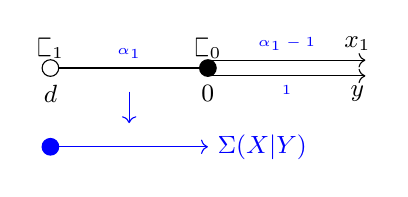
\begin{tikzpicture}[scale=1]
%edge
\draw (0,0) to (2,0);
\draw [color=blue] (1,0) node[above]{\tiny$\alpha_1$};

%C_1
\draw [fill=white] (0,0) circle[radius=3pt];
\draw (0,-0.1) node[below]{\small$d$};
\draw (0,0) node[above]{\small$\sqC_1$};

%C_0
\draw [fill=black] (2,0) circle[radius=3pt];
\draw (2,-0.1) node[below]{\small$0$};
\draw (2,0) node[above]{\small$\sqC_0$};

%x_1
\draw [->] (2,0.1) -- (4,0.1);
\draw (3.9,0.1) node[above]{\small$x_1$};
\draw [color=blue](3,0.1) node[above]{\tiny$\alpha_1-1$};

%y
\draw [->] (2,-0.1) -- (4,-0.1);
\draw (3.9,-0.1) node[below]{\small$y$};
\draw [color=blue] (3,-0.1) node[below]{\tiny$1$};

%down arrow
\draw [color=blue,->] (1,-0.3) -- (1,-0.7);

%target
\draw [color=blue,->] (0,-1) to (2,-1);
\draw [fill=blue,color=blue] (0,-1) circle[radius=3pt];
\draw [color=blue] (2,-1) node[right]{\small$\Sigma(X|Y)$};
\end{tikzpicture}
\end{center}
% Algebro-geometric picture; replaced by tropical picture.
%%%%%%%%%%%%%%%%%%%%%%%%%%%%%%%%%%%%%%%%%%%%%%%%%%%%%%%%%%%
\begin{comment}
\begin{center}
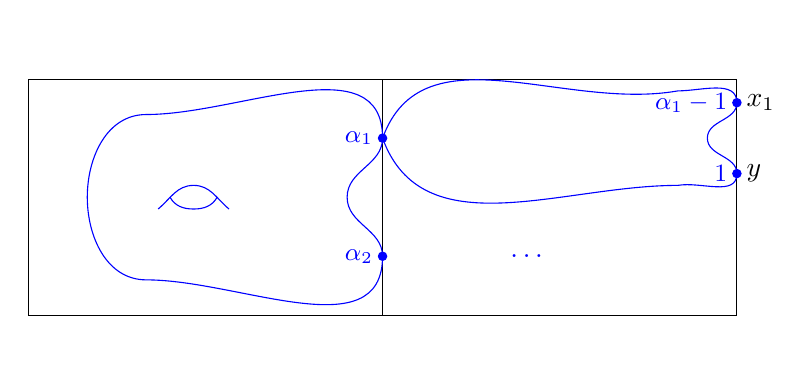
\begin{tikzpicture}[scale=1.5]
%Draw target
\draw (0,0) -- (3,0) -- (3,2) -- (0,2) -- (0,0);
\draw (3,0) -- (6,0) -- (6,2) -- (3,2) -- (3,0);

%Draw genus one curve on left-hand side
\draw [blue] (3,0.5) to [out=90,in=270] (2.7,1) to [out=90,in=270] (3,1.5) to [out=90,in=0] (1,1.7) to [out=180,in=90] (0.5,1) to [out=270,in=180] (1,0.3) to [out=0,in=270] (3,0.5);
\draw [blue] (1.1,0.9) to [out=40, in=180] (1.4,1.1) to [out=0,in=140] (1.7,0.9);
\draw [blue] (1.2,1) to [out=300, in=180] (1.4,0.9) to [out=0,in=240] (1.6,1);

%Draw nodal blobs
\draw [fill=blue,color=blue] (3,0.5) circle[radius=1pt];
\draw [color=blue] (3,0.5) node[left]{\small$\alpha_2$};
\draw [fill=blue,color=blue] (3,1.5) circle[radius=1pt];
\draw [color=blue] (3,1.5) node[left]{\small$\alpha_1$};
%Draw rational bubble with x_1 and y
\draw [blue] (3,1.5) to [out=70,in=190] (5.5,1.9) to [out=0,in=90] (6,1.8) to [out=270,in=90] (5.75,1.5) to [out=270,in=90] (6,1.2) to [out=270,in=10] (5.5,1.1) to [out=180,in=290] (3,1.5);

%Draw right-hand markings
\draw [fill=blue,color=blue] (6,1.8) circle[radius=1pt];
\draw [color=blue] (6,1.8) node[left]{\small{$\alpha_1-1$}};
\draw (6,1.8) node[right]{$x_1$};
\draw [fill=blue,color=blue] (6,1.2) circle[radius=1pt];
\draw [color=blue] (6,1.2) node[left]{\small{$1$}};
\draw (6,1.2) node[right]{$y$};

%Draw ldots
\draw [color=blue] (4,0.5) node[right]{$\ldots$};
\end{tikzpicture}
\end{center}
\end{comment}
%%%%%%%%%%%%%%%%%%%%%%%%%%%%%%%%%%%%%%%%%%%%%%%%%%%%%%%%%
with all other marked points contained on $\sqC_1$. This is isomorphic to $\VZ_{1,\alpha}(X|Y,\beta)$ and when we restrict $\tilde\gamma$ to this locus we obtain precisely the class $\gamma$ which we started with. Thus the left-hand side of \eqref{step 1 recursion} may be written as
\begin{equation*} (\alpha_1-1) I + \fgt_y^\st \left( (\alpha_1-1)\psi_1 + \ev_1^\st Y\right)  \tilde\gamma \cap [\VZ_{1,(\alpha-e_1)\cup(1)}(X|Y,\beta)]\end{equation*}
where $I$ is the invariant we are trying to compute. The second term is a forgetful relative invariant with the same degree and number of true markings (since $y$ is fictitious), and strictly smaller true tangency; hence it is recursively known. We now examine the right-hand side of \eqref{step 1 recursion}. Recall that all of the genus zero data has already been computed, so we only need to focus on the genus one pieces. First consider the type $A$ loci. The genus one piece has strictly smaller degree (and hence is recursively known) exept in the following situation (with some stable distribution of the remaining markings):
\begin{center}
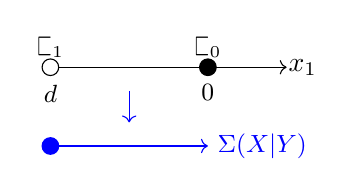
\begin{tikzpicture}[scale=1]
\draw (0,0) to (2,0);
\draw [fill=white] (0,0) circle[radius=3pt];
\draw (0,-0.1) node[below]{\small$d$};
\draw (0,0) node[above]{\small$\sqC_1$};
\draw [fill=black] (2,0) circle[radius=3pt];
\draw (2,-0.1) node[below]{\small$0$};
\draw (2,0) node[above]{\small$\sqC_0$};
\draw [->] (2,0) -- (3,0);
\draw (2.9,0) node[right]{$x_1$};

\draw [color=blue,->] (1,-0.3) -- (1,-0.7);

\draw [color=blue,->] (0,-1) to (2,-1);
\draw [fill=blue,color=blue] (0,-1) circle[radius=3pt];
\draw [color=blue] (2,-1) node[right]{\small$\Sigma(X|Y)$};
\end{tikzpicture}
\end{center}
In this situation, $C_1$ contains at most $n+1$ true markings. If it has $n-1$ or fewer, than it is known recursively. If it has exactly $n$ this means that $C_0$ contains exactly one true marking (besides $x_1$, which may be true or fictitious). We claim that in this situation we must have $y \in C_1$, since otherwise we would have a moduli space for $C_0$ given by $\ol\Mcal_{0,k}$ with $k \geq 4$, and  applying the projection formula with $\fgt_y$ we would conclude that the contribution is zero. Thus we have $y \in C_1$, and so the genus one contribution is a forgetful relative invariant with $n$ true markings, and hence is recursively known.

Finally, if $C_1$ contains exactly $n+1$ true markings, then the only additional markings on $C_0$ are fictitious, and by the same argument as in the previous paragraph there can only be one. Thus for each fictitious marked point we obtain a locus isomorphic to $\VZ_{1,\alpha}(X|Y,\beta)$ and $\tilde\gamma$ restricts to $\gamma$ here (from the point of view of computing invariants, the fictitious marked points are indistinguishable, meaning that the contributions are all the same). Thus for each fictitious marked point (of which there is at least one, namely $y$) we get a contribution of $\alpha_1 I$ to the right-hand side of \eqref{step 1 recursion}.

The contributions of the type $B$ loci only involve genus zero data and hence are known. The contributions of the type $C^0$ loci are determined by genus zero data and tautological integrals on Deligne--Mumford space, hence are also known. It remains to consider type $C^+$ loci. If the degree of the genus one piece is less than $d$ then we have a rubber invariant of strictly smaller degree. The only other possibility is that the entire curve is mapped into the divisor. In this case we may apply the projection formula with $\fgt_y$ to identify this with an integral over $\VZ_{1,m}(Y,\beta)$ for some (possibly large) number $m$ of marked points. But by assumption there is another marked point $x_0$ with all of the insertions pulled back along $\fgt_{x_0}$, so a further application of the projection formula shows that this contribution vanishes. To conclude, we may rearrange \eqref{step 1 recursion} to obtain an expression of the form
\begin{equation*} \lambda I = \text{recursively known terms} \end{equation*}
where $\lambda$ is an explicit scalar which is always nonzero; we have thus determined $I$, which completes Step 1.

\subsection*{Step 2} Consider now the absolute space $\VZ_{1,n}(Y,\beta)$ with an insertion $\gamma$, and suppose inductively that we have computed all forgetful relative invariants with $(d^\prime,n^\prime) \leq (d,n+1)$, all relative invariants and absolute invariants with $(d^\prime,n^\prime) < (d,n)$, and all special rubber invariants with $d^\prime < d$. Consider the following moduli space with $n+1$ markings:
\begin{equation*} \VZ_{1,(d,0,\ldots,0)}(X|Y,\beta). \end{equation*}
Let $x_0$ denote the relative marking and consider the integrand $\tilde\gamma$ obtained from $\gamma$ by introducing $\fgt^\st_{x_0}$ everywhere. Now recurse at $x_1$ to obtain:
\begin{equation}\label{step 2 recursion} \ev_1^\st Y \cdot \tilde\gamma \cap [\VZ_{1,(d,0,\ldots,0)}(X|Y,\beta)] = \tilde\gamma\cap[\Dcal(1)].\end{equation}
The left-hand side is a forgetful relative invariant of degree $d$ and $\leq n+1$ true markings, and so has already been computed. For the right-hand side, let us begin with loci of type $A$. The genus one contributions from each loci have $(d^\prime,n^\prime) < (d,n)$ except in the following case
\begin{center}
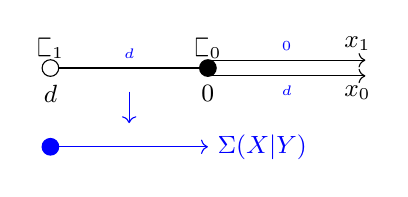
\begin{tikzpicture}[scale=1]
%edge
\draw (0,0) to (2,0);
\draw [color=blue] (1,0) node[above]{\tiny$d$};

%C_1
\draw [fill=white] (0,0) circle[radius=3pt];
\draw (0,-0.1) node[below]{\small$d$};
\draw (0,0) node[above]{\small$\sqC_1$};

%C_0
\draw [fill=black] (2,0) circle[radius=3pt];
\draw (2,-0.1) node[below]{\small$0$};
\draw (2,0) node[above]{\small$\sqC_0$};

%x_1
\draw [->] (2,0.1) -- (4,0.1);
\draw (3.9,0.1) node[above]{\small$x_1$};
\draw [color=blue](3,0.1) node[above]{\tiny$0$};

%y
\draw [->] (2,-0.1) -- (4,-0.1);
\draw (3.9,-0.1) node[below]{\small$x_0$};
\draw [color=blue] (3,-0.1) node[below]{\tiny$d$};

%down arrow
\draw [color=blue,->] (1,-0.3) -- (1,-0.7);

%target
\draw [color=blue,->] (0,-1) to (2,-1);
\draw [fill=blue,color=blue] (0,-1) circle[radius=3pt];
\draw [color=blue] (2,-1) node[right]{\small$\Sigma(X|Y)$};
\end{tikzpicture}
\end{center}
which gives a contribution of
\begin{equation*} d\cdot \gamma \cap [\VZ_{1,(d,\underbrace{0,\ldots,0}_{n-1})}(X|Y,\beta)] \footnote{(Navid) Fix formatting}\end{equation*}
to the right-hand side of \eqref{step 2 recursion}. Here $\gamma$ is the insertion we started with; the difference is that we are now considering relative maps to $(X,Y)$ with maximal tangency at $x_1$, rather than absolute maps to $Y$. The type $B$ and $C^0$ loci are recursively determined as in Step~1, and similarly the type $C^+$ loci are recursively determined except for the locus where the entire curve is mapped into the divisor. On this locus we may apply $\fgt_{x_0}$ and identify the contribution with
\begin{equation*} d^2 \cdot \gamma \cap [\VZ_{1,n}(Y,\beta)] = d^2 \cdot I \end{equation*}
where $I$ is the invariant we are trying to compute. Putting this all together, we obtain
\begin{equation}\label{step 2 recursion 2} I = (-\gamma/d) \cap [\VZ_{1,(d,\underbrace{0,\ldots,0}_{n-1})}(X|Y,\beta)] + \text{recursively known terms} \end{equation}
where on the right-hand side there are $n-1$ non-relative markings $x_2,\ldots,x_n$, and a relative marking $x_1$. We now apply the recursion again to the right-hand side, by considering the space
\begin{equation*} \VZ_{1,(d-1,1,0,\ldots,0)}(X|Y,\beta) \end{equation*}
where $x_1$ now has tangency $d-1$ and we have introduced a new marking $y$ with tangency $1$. We consider a new insertion, denoted $\tilde\gamma$ as usual, by introducing $\fgt_y^\st$ everywhere. Recursing at $x_1$ we obtain:
\begin{equation}\label{step 2 recursion 2} \left( (d-1)\psi_1 + \ev_1^\st Y \right)\cdot(-\tilde\gamma/d) \cap [\VZ_{1,(d-1,1,0,\ldots,0)}(X|Y,\beta)] = (-\tilde\gamma/d) \cap [\Dcal(1)].\end{equation}
The difference between $\psi_1$ and $\fgt_y^\st \psi_1$ is given by the locus where $x_1$ and $y$ belong to a collapsed rational bubble:
\begin{center}
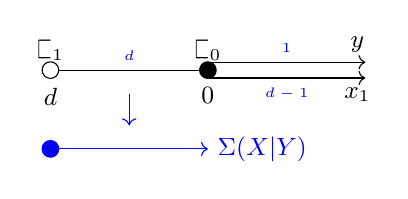
\begin{tikzpicture}[scale=1]
%edge
\draw (0,0) to (2,0);
\draw [color=blue] (1,0) node[above]{\tiny$d$};

%C_1
\draw [fill=white] (0,0) circle[radius=3pt];
\draw (0,-0.1) node[below]{\small$d$};
\draw (0,0) node[above]{\small$\sqC_1$};

%C_0
\draw [fill=black] (2,0) circle[radius=3pt];
\draw (2,-0.1) node[below]{\small$0$};
\draw (2,0) node[above]{\small$\sqC_0$};

%x_1
\draw [->] (2,0.1) -- (4,0.1);
\draw (3.9,0.1) node[above]{\small$y$};
\draw [color=blue](3,0.1) node[above]{\tiny$1$};

%y
\draw [->] (2,-0.1) -- (4,-0.1);
\draw (3.9,-0.1) node[below]{\small$x_1$};
\draw [color=blue] (3,-0.1) node[below]{\tiny$d-1$};

%down arrow
\draw [color=blue,->] (1,-0.3) -- (1,-0.7);

%target
\draw [color=blue,->] (0,-1) to (2,-1);
\draw [fill=blue,color=blue] (0,-1) circle[radius=3pt];
\draw [color=blue] (2,-1) node[right]{\small$\Sigma(X|Y)$};
\end{tikzpicture}
\end{center}
The contribution of this locus to the left-hand side of \eqref{step 2 recursion 2} is:
\begin{equation*} (d-1)\cdot(-\gamma/d) \cap [\VZ_{1,(d,\underbrace{0,\ldots,0}_{n-1})}(X|Y,\beta)].\end{equation*}
What remains on the left-hand side is a forgetful relative invariant of degree $d$ and $\leq n+1$ true markings ($y$ being the ``forgetful'' marking), hence is recursively known. On the right-hand side, the type $A$ loci are recursively known except possibly in the following special cases (with some stable distribution of the remaining non-relative markings):
\begin{center}
\begin{minipage}{0.4\textwidth}
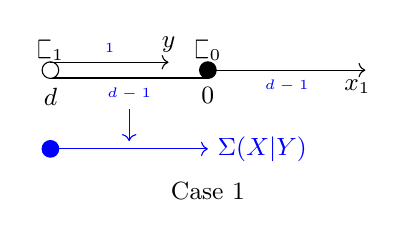
\begin{tikzpicture}[scale=1]
%edge
\draw (0,-0.1) to (2,-0.1);
\draw [color=blue] (1,-0.1) node[below]{\tiny$d-1$};

%C_1
\draw [fill=white] (0,0) circle[radius=3pt];
\draw (0,-0.1) node[below]{\small$d$};
\draw (0,0) node[above]{\small$\sqC_1$};

%C_0
\draw [fill=black] (2,0) circle[radius=3pt];
\draw (2,-0.1) node[below]{\small$0$};
\draw (2,0) node[above]{\small$\sqC_0$};

%x_1
\draw [->] (0,0.1) -- (1.5,0.1);
\draw (1.5,0.1) node[above]{\small$y$};
\draw [color=blue](0.75,0.1) node[above]{\tiny$1$};

%y
\draw [->] (2,0) -- (4,0);
\draw (3.9,0) node[below]{\small$x_1$};
\draw [color=blue] (3,0) node[below]{\tiny$d-1$};

%down arrow
\draw [color=blue,->] (1,-0.5) -- (1,-0.9);

%target
\draw [color=blue,->] (0,-1) to (2,-1);
\draw [fill=blue,color=blue] (0,-1) circle[radius=3pt];
\draw [color=blue] (2,-1) node[right]{\small$\Sigma(X|Y)$};

\draw (2,-1.3) node[below]{\small{Case 1}};
\end{tikzpicture}
\end{minipage}
\begin{minipage}{0.4\textwidth}
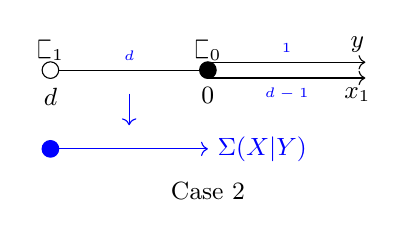
\begin{tikzpicture}[scale=1]
%edge
\draw (0,0) to (2,0);
\draw [color=blue] (1,0) node[above]{\tiny$d$};

%C_1
\draw [fill=white] (0,0) circle[radius=3pt];
\draw (0,-0.1) node[below]{\small$d$};
\draw (0,0) node[above]{\small$\sqC_1$};

%C_0
\draw [fill=black] (2,0) circle[radius=3pt];
\draw (2,-0.1) node[below]{\small$0$};
\draw (2,0) node[above]{\small$\sqC_0$};

%x_1
\draw [->] (2,0.1) -- (4,0.1);
\draw (3.9,0.1) node[above]{\small$y$};
\draw [color=blue](3,0.1) node[above]{\tiny$1$};

%y
\draw [->] (2,-0.1) -- (4,-0.1);
\draw (3.9,-0.1) node[below]{\small$x_1$};
\draw [color=blue] (3,-0.1) node[below]{\tiny$d-1$};

%down arrow
\draw [color=blue,->] (1,-0.3) -- (1,-0.7);

%target
\draw [color=blue,->] (0,-1) to (2,-1);
\draw [fill=blue,color=blue] (0,-1) circle[radius=3pt];
\draw [color=blue] (2,-1) node[right]{\small$\Sigma(X|Y)$};

\draw (2,-1.3) node[below]{\small{Case 2}};
\end{tikzpicture}
\end{minipage}
\end{center}
In Case 1 the contribution from $C_1$ is a forgetful relative invariant with $\leq n$ true markings, hence is recursively known. In Case 2, we first note that there cannot be any more markings on $C_0$ (since otherwise we could apply $\fgt_y$ and conclude that the contribution vanishes). Thus we obtain a single locus, which contributes precisely
\begin{equation*} d\cdot(-\gamma/d) \cap [\VZ_{1,(d,\underbrace{0,\ldots,0}_{n-1})}(X|Y,\beta)] = -\gamma\cap[\VZ_{1,(d,\underbrace{0,\ldots,0}_{n-1})}(X|Y,\beta)]\end{equation*}
which gives us the first term on the right-hand side of \eqref{step 2 recursion 2}. As usual the type $B$ and $C^0$ contributions are known recursively, and the only type $C^+$ contribution not known recursively occurs when the entire curve is mapped into the divisor, in which case we apply $\fgt_y$ to calculate the contribution as:
\begin{equation*} (-\gamma/d) \cap [\VZ_{1,n}(Y,\beta)] = -I/d.\end{equation*}
Substituting into \eqref{step 2 recursion 2} we end up with
\begin{equation*} I(1-d^{-1}) = \text{recursively known terms} \end{equation*}
which completes the recursion step as long as $d \neq 1$. But since $\VZ_{1,n}(H,1)=\emptyset$ it follows that $\VZ_{1,n}(Y,\beta)=\emptyset$ if $d=Y\cdot\beta=1$, so we may always assume $d \geq 2$ in the recursion.

\subsection*{Step 3} Now suppose we are given a relative space $\VZ_{1,\alpha}(X|Y,\beta)$ with an insertion $\gamma$, and suppose inductively that we have computed all forgetful relative invariants with $(d^\prime,n^\prime) \leq (d,n+1)$, all absolute invariants with $(d^\prime,n^\prime) \leq (d,n)$, all relative invariants with $(d^\prime,n^\prime,t^\prime)<(d,n,t)$ and all rubber invariants with $d^\prime < d$. Choose a true marking $x_1$ with $\alpha_1 \geq 1$ and consider the moduli space
\begin{equation*} \VZ_{1,(\alpha-e_1)\cup(1)}(X|Y,\beta) \end{equation*}
where $y$ is the newly-introduced marking. As usual consider the insertion $\tilde\gamma$ obtained from $\gamma$ by introducing $\fgt_y$ everywhere. Recursing at $x_1$ we obtain:
\begin{equation*} \left( (\alpha_1-1)\psi_1 + \ev_1^\st H\right) \tilde\gamma \cap [\VZ_{1,(\alpha-e_1)\cup(1)}(X|Y,\beta)] = \tilde\gamma \cap [\Dcal(1)].\end{equation*}
The left-hand side is a relative invariant with the same degree and number of true markings, but smaller true tangency: hence it is recursively known. On the right-hand side, the type $A$ contributions are recursively known except for those of the following form

\begin{center}
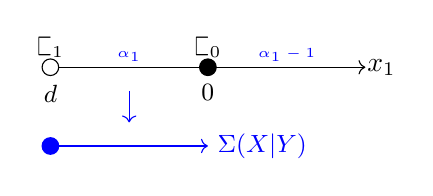
\begin{tikzpicture}[scale=1]
\draw (0,0) to (2,0);
\draw [color=blue] (1,-0.05) node[above]{\tiny$\alpha_1$};
\draw [fill=white] (0,0) circle[radius=3pt];
\draw (0,-0.1) node[below]{\small$d$};
\draw (0,0) node[above]{\small$\sqC_1$};
\draw [fill=black] (2,0) circle[radius=3pt];
\draw (2,-0.1) node[below]{\small$0$};
\draw (2,0) node[above]{\small$\sqC_0$};
\draw [->] (2,0) -- (4,0);
\draw (3.9,0) node[right]{$x_1$};
\draw [color=blue] (3,-0.05) node[above]{\tiny$\alpha_1-1$};

\draw [color=blue,->] (1,-0.3) -- (1,-0.7);

\draw [color=blue,->] (0,-1) to (2,-1);
\draw [fill=blue,color=blue] (0,-1) circle[radius=3pt];
\draw [color=blue] (2,-1) node[right]{\small$\Sigma(X|Y)$};
\end{tikzpicture}
\end{center}
where $C_0$ contains a single fictitious marking (if it had multiple fictitious markings then the contribution would vanish by projection formula) and all the other markings are on $C_1$. Thus for each fictitious marking we get a contribution of $\alpha_1 I$ where $I$ is the invariant we are trying to compute. Note that $\alpha_1 \neq 0$, and that this term appears at least once since $y$ is a fictitious marking; so we get a nonzero multiple of $I$.

As usual the type $B$ and $C^0$ contributions are recursively known. The type $C^+$ contributions are determined by lower-degree rubber invariants, except for when the whole curve is mapped into $Y$; however in this case we may apply $\fgt_y$ to identify the contribution with an absolute invariant of $Y$ with degree $d$ and $n$ markings, which is also recursively known. Thus we have determined the invariant $I$.

\subsection*{Step 4} Finally, consider a rubber space $\VZ_{1,\alpha}(P|Y_0+Y_\infty,\beta)_{\Gm}$ with insertion $\gamma$. Suppose inductively that we have computed all absolute and relative invariants with $d^\prime \leq d$ and all rubber invariants with $(d^\prime,n^\prime,m^\prime) < (d,n,m)$.

We first note the following important reduction: if there exists a relative marking $x_k$ such that all insertions are pulled back along $\fgt_{k}$, then we may apply the projection formula, together with the fact that
\begin{equation*} (\fgt_{k})_\st [\VZ_{1,\alpha}(P|Y_0+Y_\infty,\beta)_{\Gm}] = \alpha_k^2 \cdot [\VZ_{1,n+m-1}(Y,\beta)] \end{equation*}
to identify the rubber invariant with a multiple of a reduced invariant of $Y$, which has the same degree and hence is known recursively.

We will deal with the general case by reducing to the one above. Consider the moduli space
\begin{equation*}\label{step 4 recursion space} \VZ_{1,\alpha\cup (0)}(P|Y_0+Y_\infty,\beta)_{\Gm}\end{equation*}
obtained by introducing a marked point $y$ with no tangency. Let $x_1$ be a positive-tangency marking (such a marking always exists since $d \geq 2$) and let $\tilde\gamma$ be the insertion obtained from $\gamma$ by replacing $\ev_1$ and $\psi_1$ by $\ev_y$ and $\psi_y$, and then introducing $\fgt_{1}^\st$ everywhere.

We will make use of a recursion formula for rubber spaces analogous to the recursion formula for relative spaces used in Steps 1--3. Following \cite{EKatz}, there is a line bundle $L_y^{\not\in \operatorname{bot}}$ on $\VZ_{1,\alpha\cup (0)}(P|Y_0+Y_\infty,\beta)_{\Gm}$, together with a section $s_y^{\not\in\operatorname{bot}}$ whose vanishing locus consists of the locus $\Dcal(y)$ of rubber maps where $y$ is not mapped into the bottom level of the expanded target. As in \S \ref{}, we can give a logarithmic interpretation of this: it corresponds to the piecewise-linear function on the tropical moduli space which associates, to every rubber tropical map, the distance between $\varphi(\sqC_y)$ and the leftmost vertex of the tropical target, where $\sqC_y$ is the vertex of the source curve containing the flag corresponding to $y$. Using this tropical description, we may easily calculate the vanshing orders of $s_y^{\not\in\operatorname{bot}}$ along the various components of $\Dcal(y)$, and show that $\cchern_1(L_y^{\not\in\operatorname{bot}}) = \Psi_0 - \ev_y^\st Y$ (see also \cite{EKatzLB}, where similar results in the non-reduced setting are obtained, using different methods). From this, we obtain a rubber recursion formula
\begin{equation}\label{step 4 recursion} (\Psi_0 - \ev_y^\st Y) \tilde\gamma \cap [\VZ_{1,\alpha\cup(0)}(P|Y_0+Y_\infty,\beta)_{\Gm}] = \tilde\gamma \cap [\Dcal(y)]\end{equation}
where the fundamental class $[\Dcal(y)]$ is weighted by vanishing orders on the components. We will first show that the left-hand side is recursively known. By construction the class $\tilde\gamma$ is pulled back via $\fgt_{1}^\st$, and the same is true for $\ev_y^\st Y$. It remains to examine $\Psi_0$. If there exists a negative-tangency marking $x_2$, then we have \cite[Construction 5.1.17]{GathmannThesis}
\begin{equation*}\label{Psi0 formula} \Psi_0 = -\alpha_2 \hat\psi_2 - \ev_2^\st Y \end{equation*}
where $\hat\psi_2$ is a \emph{non-collapsed} psi class. (If there are no negative-tangency markings, then the construction given in \cite[\S 1.5.2]{MaulikPandharipande} shows that $\Psi_0=0$.) Now, $\hat\psi_2 - \psi_2$ is given by the loci where $x_2$ belongs to a trivial bubble. This entails a splitting of the curve into pieces, each of which contributes a rubber integral. Typically each of these pieces will have $(g^\prime,d^\prime,n^\prime,m^\prime) < (1,d,n,m)$ and hence be recursively known. The one exception is when all of the genus and degree is concentrated on the top level of the expansion, with the bottom level containing only a single non-relative marking in addition to all the negative-tangency markings. But in this case the contribution is a rubber invariant where all of the insertions are pulled back via $\fgt_1^\st$, and hence we may apply the projection formula to identify this with an absolute invariant of $Y$ which is recursively known. We conclude that, up to recursively knwon terms, we may replace $\hat\psi_2$ by $\psi_2$ in the left-hand side of \eqref{step 4 recursion}. If we now compare $\psi_2$ with $\fgt_1^\st \psi_2$ we see that the difference is given by the locus where $x_1$ and $x_2$ belong to a collapsed rational piece. The contribution of this locus consists of rubber invariant with strictly fewer relative markings, and hence is recursively known. So up to recursively-known terms \eqref{step 4 recursion} becomes
\begin{equation*} \fgt_1^\st (-\alpha_2\psi_2 - \ev_y^\st Y)\tilde\gamma \cap [\VZ_{1,\alpha\cup(0)}(P|Y_0+Y_\infty,\beta)_{\Gm}] = \tilde\gamma\cap[\Dcal(y)]\end{equation*}
and now the left-hand side is also recursively known, by the projection formula. Let us now examine the right-hand side. The components of $\Dcal(y)$ are indexed by splittings of the curve, and certainly the contributions are recursively known unless there is a piece of the curve carrying all of the genus and degree, so we may restrict to examining these contributions.

Let us denote the piece of the curve carrying all of the genus and degree by $C^\prime\subseteq C$. If $C^\prime$ is mapped to top level, then either it contains $x_1$, in which case we apply $\fgt_1$ to compute the contribution, or it does not contains $x_1$, in which case it has fewer than $n$ relative markings and is known recursively.  If on the other hand $C^\prime$ is not mapped to top level, then generically it is mapped to the bottom level (since generically the circuit is not contracted on this locus, so the desingularisation process does nothing). One possible contribution is given by the following locus
\begin{center}
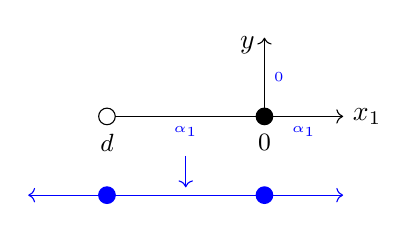
\begin{tikzpicture}[scale=1]
%edge
\draw (0,0) to (2,0);
\draw [color=blue] (1,0) node[below]{\tiny$\alpha_1$};

%C_1
\draw [fill=white] (0,0) circle[radius=3pt];
\draw (0,-0.1) node[below]{\small$d$};

%y
\draw [->] (2,0) -- (2,1);
\draw (2,0.9) node[left]{$y$};
\draw [color=blue] (2,0.5) node[right]{\tiny$0$};

%x_1
\draw [->] (2,0) -- (3,0);
\draw (3,0) node[right]{$x_1$};
\draw [color=blue] (2.5,0) node[below]{\tiny$\alpha_1$};

%C_0
\draw [fill=black] (2,0) circle[radius=3pt];
\draw (2,-0.1) node[below]{\small$0$};

%down arrow
\draw [color=blue,->] (1,-0.5) -- (1,-0.9);

%target
\draw [color=blue] (0,-1) to (2,-1);
\draw [fill=blue,color=blue] (0,-1) circle[radius=3pt];
\draw [fill=blue,color=blue] (2,-1) circle[radius=3pt];
\draw [color=blue,->] (2,-1) -- (3,-1);
\draw [color=blue,->] (0,-1) -- (-1,-1);
\end{tikzpicture}
\end{center}
which contributes a nonzero multiple of the invariant $I$ we are trying to compute. For the other possibilities, first note that, unless every component at the top level contains a single positive-tangency marking and a single node (together with possibly some tangency-zero markings), then $C^\prime$ has fewer than $n$ relative markings and hence the contribution is known recursively. On the other hand, if any non-relative marking other than $y$ is mapped to the top level, $C^\prime$ has $\leq n$ relative markings and less than $m$ non-relative markings, and hence again the contribution is known recursively. The only remaining possibilities are when $x_1$ is replaced by another positive-tangency marking $x_k$ in the above picture; but then the contribution can be calculated by applying the projection formula to $\fgt_{1}$. We therefore conclude that the only contribution to the right-hand side of \eqref{step 4 recursion} which is not known recursively is a nonzero multiple of the invariant we were trying to compute. This completes the recursion step.

\newpage

\section{Description of the logarithmic strata}
\noindent Let $\VZ = \VZ_{1,\alpha}(\PP^N|H,d)$ and let $\Acal$ denote the Artin fan of $\VZ$. Since the map of log stacks
\begin{equation*} \VZ \to \Acal \end{equation*}
is smooth, we see that the codimension-$k$ logarithmic strata in $\VZ$ are in bijective correspondence (via pull-back) with the codimension-$k$ logarithmic strata in $\Acal$. The logarithmic strata in $\Acal$, on the other hand, have a purely combinatorial description (at least locally) in terms of the associated moduli spaces of tropical maps, coming from the fact that $\VZ$ is a logarithmic blow-up of the usual moduli space of log stable maps. In this section we discuss this circle of ideas, and show how it plays out in a number of examples.

\subsection{Blowing up the Artin fan}
Let $\Mcal = \ol{\Mcal}^{\op{log}}_{1,\alpha}(\PP^N|H,d)$ denote the Abramovich--Chen--Gross--Siebert moduli space of log stable maps. Recall that $\VZ$ is obtained as a closed substack of a log modification
\begin{equation*} \widetilde{\VZ} \to \Mcal .\end{equation*}
Since the map $\VZ \hookrightarrow \widetilde{\VZ}$ is strict, the Artin fan $\Acal$ of $\VZ$ is locally isomorphic to the Artin fan of $\widetilde{\VZ}$ (with the latter being, in general, larger)\footnote{(Navid) Make this more precise}. Since the following discussion is entirely local, we will ignore the distinction between the two, and pretend as though $\Acal$ is the Artin fan of $\widetilde{\VZ}$. There is then a commuting square:
\bcd
\widetilde{\VZ} \ar[r] \ar[d] & \Mcal \ar[d] \\
\Acal \ar[r] & \Acal_{\Mcal}.
\ecd
Note that neither of the vertical maps are smooth, since the moduli spaces on the top row are not log smooth. The construction of $\widetilde{\VZ} \to \Mcal$ as the log modification obtained by imposing an alignment condition gives us a combinatorial description of the map $\Acal \to \Acal_{\Mcal}$ which we will use to study $\Acal$. Recall that $\Acal_\Mcal$ is locally isomorphic to the stack quotient
\begin{equation*} \left[ \Spec \kfield[Q] / \Spec\kfield [Q^{\gp}] \right]\end{equation*}
where $Q$ is a monoid giving a\footnote{(Navid) Neat?} local chart for $\Mcal$, which we may take to be the minimal monoid of \cite[\S 1.5]{GrossSiebertLog}. The real dual $Q^\vee_{\RR} = \Hom(Q,\RR_{\geq 0})$ of this monoid can be viewed as a moduli space of tropical maps; see \cite[Remark 1.12]{GrossSiebertLog}. We call this \emph{the tropical moduli space}; contained in the tropical moduli space are the edge lengths of the associated tropical curve (corresponding to the smoothing parameters of the nodes of the logarithmic curve). Since the alignment condition amounts to imposing a partial ordering amongst certain sums of these edge lengths, it produces a polyhedral decomposition of the tropical moduli space, into chambers where different partial order relations hold. If we only consider the integral points, this produces a polyhedral decomposition of the cone $Q^\vee = \Hom(Q,\N)$. Dualising, we obtain a toric blow-up
\begin{equation*} Z \to \Spec \kfield[Q] \end{equation*}
which, since it is equivariant, descends to a morphism of the associated zero-dimensional stacks:
\begin{equation*} \left[Z/T_Z \right] \to \left[ \Spec \kfield[Q] / \Spec\kfield [Q^{\gp}] \right]. \end{equation*}
This gives a local description of the map $\Acal \to \Acal_\Mcal$ and in particular of the Artin fan $\Acal$. By the orbit-cone correspondence, the codimension-$k$ strata of $\Acal$ which intersect this open locus correspond to the $k$-dimensional cones in the polyhedral decomposition of $Q^\vee$ described above. These can be understood entirely in terms of tropical combinatorics. This is best explained through a number of examples, which we now present.

\subsection{Examples of logarithmic strata} In these examples we will proceed as follows: we will start by fixing an element of the ordinary moduli space $\Mcal$ of log stable maps. We will then compute the associated tropical moduli space, giving a description of $\Acal_\Mcal$ local to our chosen element. We will then describe the necessary polyhedral subdivison, and thus give a description of $\Acal$ in a neighbourhood of the preimage in $\VZ$ of our chosen element of $\Mcal$. Finally we will use this to describe the logarithmic strata which intersect this neighbourhood.
\begin{example} Consider an element of $\Mcal$ whose associated tropical map has the following combinatorial type:
\begin{center}
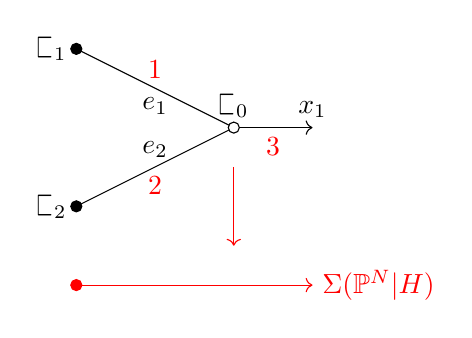
\begin{tikzpicture}
\draw [fill] (0,3) circle[radius=2pt];
\draw (0,3) node[left]{$\sqC_1$};
\draw (0,3) -- (2,2);
\draw (1,2.5) node[above,color=red]{$1$};
\draw (1,2.5) node[below]{$e_1$};

\draw [fill] (0,1) circle[radius=2pt];
\draw (0,1) node[left]{$\sqC_2$};
\draw (0,1) -- (2,2);
\draw (1,1.5) node[below,color=red]{$2$};
\draw (1,1.5) node[above]{$e_2$};

\draw [->] (2,2) -- (3,2);
\draw (3,2) node[above]{$x_1$};
\draw (2.5,2) node[below,red]{$3$};

\draw [fill=white] (2,2) circle[radius=2pt];
\draw (2,2) node[above]{$\sqC_0$};

\draw [->,color=red] (2,1.5) -- (2,0.5);

\draw [->,color=red] (0,0) -- (3,0);
\draw (0,0) [fill=red,color=red] circle[radius=2pt];
\draw (3,0) node[right,color=red]{$\Sigma(\PP^N|H)$};
\end{tikzpicture}
\end{center}
Here each edge (corresponding to a node of the curve) has a length $e_i$ and an expansion factor $u_i$ (indicated in red). The moduli space of such tropical maps is generated by the edge lengths $e_1$ and $e_2$
\begin{equation*} (\RR_{\geq 0})_{e_1} \times (\RR_{\geq 0})_{e_2} \end{equation*}
subject to the continuity condition $e_1=2e_2$. So the tropical moduli space is simply $\RR_{\geq 0}$ generated by $e_2$. Note that for any $e_2 > 0$ (i.e. on the interior of the cone) we have:
\begin{equation*} \lambda(\sqC_2) = e_2 = e_1/2 < e_1 = \lambda(\sqC_1). \end{equation*}
Thus, any logarithmic map with combinatorial type given by the above picture is automatically aligned. This means that the map $\VZ \to \Mcal$ is an isomorphism in a neighbourhood of our chosen element (there is no blowing up necessary). Indeed, the tropical moduli space is $\RR_{\geq 0}$ and this cone does not admit a polyhedral subdivision (there is no non-trivial toric blow-up of $\Aaff^1$).
\end{example}

\begin{example}
Consider now an element of $\Mcal$ whose associated tropical map has the corresponding combinatorial type:
\begin{center}
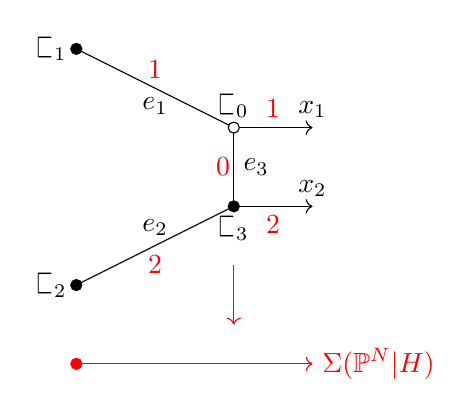
\begin{tikzpicture}
\draw [fill] (0,4) circle[radius=2pt];
\draw (0,4) node[left]{$\sqC_1$};
\draw (0,4) -- (2,3);
\draw (1,3.5) node[above,color=red]{$1$};
\draw (1,3.5) node[below]{$e_1$};

\draw [fill] (0,1) circle[radius=2pt];
\draw (0,1) node[left]{$\sqC_2$};
\draw (0,1) -- (2,2);
\draw (1,1.5) node[below,color=red]{$2$};
\draw (1,1.5) node[above]{$e_2$};

\draw [->] (2,3) -- (3,3);
\draw (3,3) node[above]{$x_1$};
\draw (2.5,3) node[above,red]{$1$};

\draw (2,3) -- (2,2);
\draw [fill] (2,2) circle[radius=2pt];
\draw (2,2.5) node[right]{$e_3$};
\draw (2.075,2.5) node[left,red]{$0$};
\draw (2,2) node[below]{$\sqC_3$};

\draw [->] (2,2) -- (3,2);
\draw (3,2) node[above]{$x_2$};
\draw (2.5,2) node[below,red]{$2$};

\draw [fill=white] (2,3) circle[radius=2pt];
\draw (2,3) node[above]{$\sqC_0$};

\draw [->,color=red] (2,1.25) -- (2,0.5);

\draw [->,color=red] (0,0) -- (3,0);
\draw (0,0) [fill=red,color=red] circle[radius=2pt];
\draw (3,0) node[right,color=red]{$\Sigma(\PP^N|H)$};
\end{tikzpicture}
\end{center}
As before, expansion factors are indicated in red and the edge lengths are $e_1,e_2,e_3$. The tropical moduli space is $\RR_{\geq 0}^3$ generated by these three lengths, subject to the continuity condition $e_1=2e_2$. Thus the moduli space is isomorphic to $\RR_{\geq 0}^2$ generated by $e_2$ and $e_3$. In order to have an alignment, at least one of $\lambda(\sqC_1)$ and $\lambda(\sqC_2)$ must be equal to the radius $\delta$. Note that
\begin{align*} \lambda(\sqC_1) & = e_1 = 2e_2 \\
\lambda(\sqC_2) & = e_2 + e_3\end{align*}
and without more information we cannot say which of these is larger. The subdivision of $(\RR_{\geq 0})^2$ is obtained by dividing the cone into regions where different order relations hold amongst the distances $\lambda(\sqC_1),\lambda(\sqC_2),\lambda(\sqC_3)$. The walls of this subdivison correspond to where some of these distances are equal. Note that in this setting we always have $\lambda(\sqC_2) > \lambda(\sqC_3)$ (at least, as long as we remain in the interior of the cone). The remaining possibilities are:
\begin{align*} \lambda(\sqC_1) & = \lambda(\sqC_3) \qquad (\Leftrightarrow e_1 = e_3 \Leftrightarrow 2e_2 = e_3) \\
\lambda(\sqC_1) & = \lambda(\sqC_2) \qquad (\Leftrightarrow e_1 = e_2 + e_3 \Leftrightarrow e_2 = e_3). \end{align*}
Thus, the subdivision of the tropical moduli space $(\RR_{\geq 0}^2)_{e_2 e_3}$ is given by:
\begin{center}
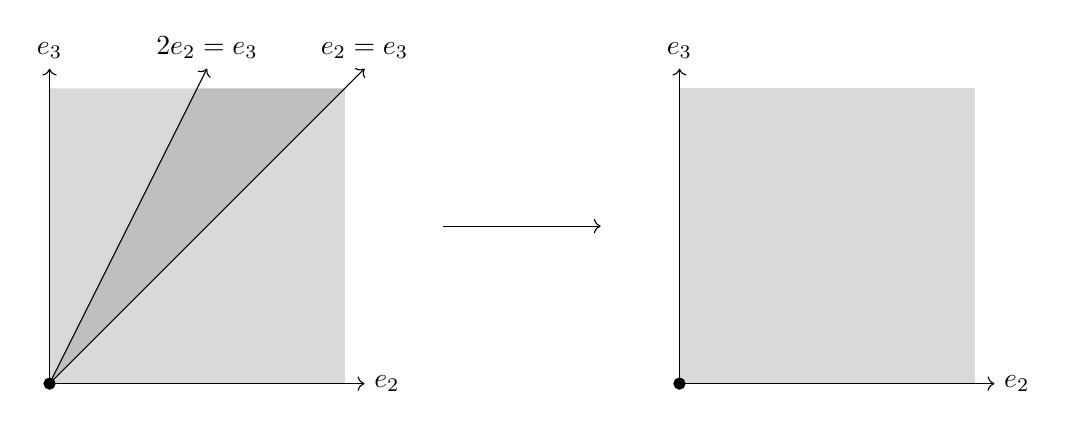
\begin{tikzpicture}[scale=1]
% Right-hand box
\fill [fill=gray!30!white] (5,0) -- (8.75,0) -- (8.75,3.75) -- (5,3.75) -- cycle;
\draw [fill] (5,0) circle[radius=2pt];
\draw [->] (5,0) -- (9,0);
\draw (9,0) node[right]{$e_2$};
\draw [->] (5,0) -- (5,4);
\draw (5,4) node[above]{$e_3$};

% Left-hand box
\fill [fill=gray!30!white] (-3,0) -- (0.75,0) -- (0.75,3.75) -- cycle;
\fill [fill=gray!50!white] (-3,0) -- (0.75,3.75) -- (-1.125,3.75) -- cycle;
\fill [fill=gray!30!white] (-3,0) -- (-1.125,3.75) -- (-3,3.75) -- cycle;
\draw [fill] (-3,0) circle[radius=2pt];
\draw [->] (-3,0) -- (1,0);
\draw (1,0) node[right]{$e_2$};
\draw [->] (-3,0) -- (-3,4);
\draw (-3,4) node[above]{$e_3$};

% 2e_2=e_3 line
\draw [->] (-3,0) -- (-1,4);
\draw (-1,4) node[above]{$2e_2=e_3$};

% e_2=e_3 line
\draw [->] (-3,0) -- (1,4);
\draw (1,4) node[above]{$e_2=e_3$};

% arrow
\draw [->] (2,2) -- (4,2);
\end{tikzpicture}
\end{center}
The cones of the subdivison index the logarithmic strata in a neighbourhood of the preimage in $\VZ$ of our chosen element of $\Mcal$. These can be described as follows:
\begin{center}
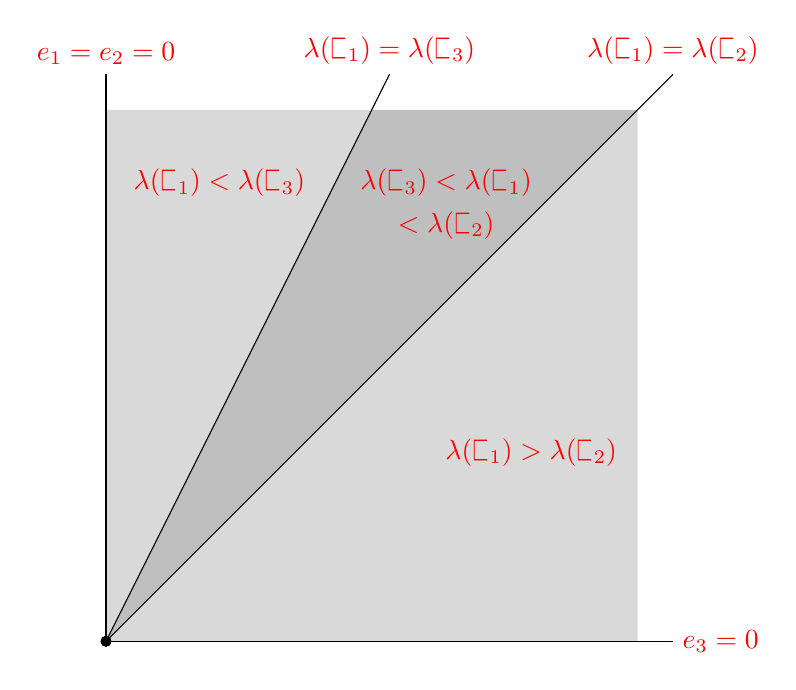
\begin{tikzpicture}[scale=1.8]
% Left-hand box
\fill [fill=gray!30!white] (-3,0) -- (0.75,0) -- (0.75,3.75) -- cycle;
\fill [fill=gray!50!white] (-3,0) -- (0.75,3.75) -- (-1.125,3.75) -- cycle;
\fill [fill=gray!30!white] (-3,0) -- (-1.125,3.75) -- (-3,3.75) -- cycle;
\draw [fill] (-3,0) circle[radius=1pt];
\draw (-3,0) -- (1,0);
\draw (1,0) node[right,red]{$e_3=0$};
\draw (-3,0) -- (-3,4);
\draw (-3,4) node[above,red]{$e_1=e_2=0$};

% 2e_2=e_3 line
\draw (-3,0) -- (-1,4);
\draw (-1,4) node[above,red]{$\lambda(\sqC_1)=\lambda(\sqC_3)$};

% e_2=e_3 line
\draw (-3,0) -- (1,4);
\draw (1,4) node[above,red]{$\lambda(\sqC_1)=\lambda(\sqC_2)$};

\draw (0,1.5) node[below,red]{$\lambda(\sqC_1) > \lambda(\sqC_2)$};

\draw (-0.6,3.4) node[below,red]{$\lambda(\sqC_3) < \lambda(\sqC_1)$};
\draw (-0.6,3.1) node[below,red]{$< \lambda(\sqC_2)$};

\draw (-2.2,3.4) node[below,red]{$\lambda(\sqC_1) < \lambda(\sqC_3)$};
\end{tikzpicture}
\end{center}
There are four codimension--$1$ logarithmic strata of $\VZ$ intersecting our chosen neighbourhood, corresponding to the rays in the above picture. Two of these -- those corresponding to the rays labeled $\{ e_1=e_2=0 \}$ and $\{ e_3=0 \}$ -- are the proper transforms of codimension--$1$ strata in $\Mcal$. These strata consist of log stable maps where some of the tropical edge lengths are equal to zero, meaning that the corresponding nodes have been smoothed. Notice that although the curve has three nodes, there are only two such strata: the nodes $q_1$ and $q_2$ cannot be smoothed independently because of the relation $e_1=2e_2$.

The remaining two codimension--$1$ strata in $\VZ$ -- corresponding to the interior rays in the above picture -- consist of log stable maps where some of the vertex distances become equal. Here none of the nodes are smoothed. From the construction of the subdivision, we see that both these strata map onto a codimension--$2$ stratum of $\Mcal$ (namely, the locus in which all of the nodes persist); this coheres with the fact that they should be thought of as exceptional loci of the blow-up. The extra dimension of moduli comes from the choice of alignment.

Finally, there are three codimension--$2$ strata, corresponding to different \emph{strict} orderings of the vertex distances. Note that the divisorial strata corresponding to $\{e_1=e_2=0\}$ and $\{e_3=0\}$, which intersected in $\Mcal$, no longer intersect in $\VZ$, since we have blown up. The picture is something like:
\begin{center}
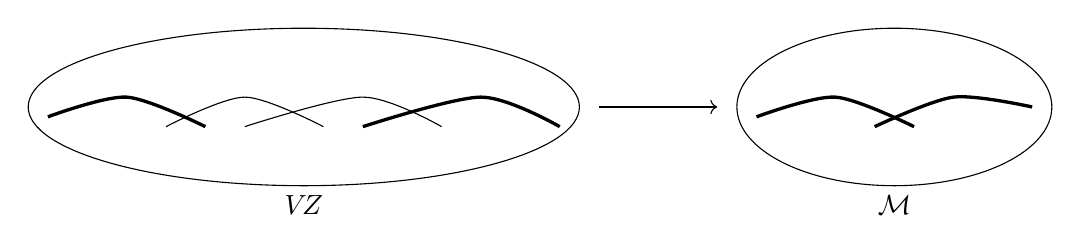
\begin{tikzpicture}[scale=0.5]
\draw (-6.5,0.5) ellipse (4 and 2);
\draw (-6.5,-1.5) node[below]{$\Mcal$};
\draw [very thick] plot [smooth] coordinates{(-10,0.25) (-8,0.75) (-6,0)};
\draw [very thick] plot [smooth] coordinates{(-7,0) (-5,0.75) (-3,0.5)};

\draw (-21.5,0.5) ellipse (7 and 2);
\draw (-21.5,-1.5) node[below]{$\VZ$};
\draw [very thick] plot [smooth] coordinates{(-28,0.25) (-26,0.75) (-24,0)};
\draw plot [smooth] coordinates{(-25,0) (-23,0.75) (-21,0)};
\draw plot [smooth] coordinates{(-23,0) (-20,0.75) (-18,0)};
\draw [very thick] plot [smooth] coordinates{(-20,0) (-17,0.75) (-15,0)};

\draw [->] (-14,0.5) -- (-11,0.5);
\end{tikzpicture}
\end{center}

\end{example}

\subsection{Global logarithmic strata}
In the previous subsections we used tropical geometry to identify the logarithmic strata of $\VZ=\VZ_{1,\alpha}(\PP^N|H,d)$ local to the preimage of a point in $\Mcal$. In fact, the whole discussion carries over if we replace a point in $\Mcal$ by a locally closed logarithmic stratum: the key observation is simply that the tropical moduli space does not vary if we move inside a locally closed logarithmic stratum, so the subdivision process makes sense over that whole stratum. This fact will allow us to describe the logarithmic strata of $\VZ$ globally.

\subsubsection{Logarithmic strata of $\Mcal$} The locally closed logarithmic strata of $\Mcal$ consist of loci where the combinatorial type of the associated tropical curve is constant\footnote{(Navid) Reference for this?}. This is because the combinatorial type determines the minimal monoid $Q$, which coincides with the stalk of the ghost sheaf on $\Mcal$.

If we have two strata $\Scal_1$ and $\Scal_2$ corresponding to combinatorial types $\Delta_1$ and $\Delta_2$, then $\Scal_2$ is contained in the closure of $\Scal_1$ if and only if the combinatorial type $\Delta_1$ is obtained from $\Delta_2$ by a process of generisation: namely, by contracting some edges (i.e. smoothing some nodes) and moving some of the vertices from the interior $\RR_{>0} \subseteq \RR_{\geq 0}$ of the tropicalisation $\Sigma(\PP^N|H)$ to the vertex $0 \in \RR_{\geq 0}$ (i.e. moving some components of the curve outside $H$). This allows us to completely describe the dual intersection complex of the logarithmic strata of $\Mcal$.

Note that we are \emph{not} able to easily read off the codimension of a logarithmic stratum from the combinatorial data: the codimension of the associated stratum in the Artin fan $\Acal_\Mcal$ is given by the dimension of the tropical moduli space, but the map $\Mcal\to\Acal_\Mcal$ is not smooth (since $\Mcal$ is not log smooth) so we are not able to say anything about the locus in $\Mcal$. 

\subsubsection{Logarithmic strata of $\VZ$}
Now let us pick a stratum $\Scal \subseteq \Mcal$ indexed by a combinatorial type $\Delta$ and with associated monoid $Q$. We may choose a sufficiently small open neighbourhood of $\Scal$ which only intersects logarithmic strata $\Scal^\prime$ which contain $\Scal$ in their closures. The previous discussion then shows that if we pick any point in this open neighbourhood, the combinatorial type of the associated tropical curve is obtained from $\Delta$ by contracting some edges and specialising some vertices. Thus we see that the associated map on tropical moduli spaces is injective, and so the generisation map on the level of ghost sheaves is surjective. This allows us to produce a chart on the open neighbourhood of $\Scal$ with monoid given by $Q$.

The discussion in the previous subsections then applies \emph{mutatis mutandis} to this open set, giving a description of the logarithmic strata of $\VZ$ which intersect an open neighbourhood of the preimage of $\Scal$. Since log strata must map to log strata, this gives a procedure for enumerating all of the locally closed logarithmic strata of $\VZ$, namely:\medskip
\begin{enumerate}
\item Enumerate the locally closed logarithmic strata of $\Mcal$ by enumerating all possible combinatorial types of tropical curves with the given numerical data. The dual intersection complex of these strata is specified by generisation of combinatorial types, as described earlier.\medskip
\item For each locally closed stratum $\Scal\subseteq \Mcal$ identify the tropical moduli space $Q^\vee_{\RR}$ associated to the given combinatorial type, and perform the subdivision specified by the alignment condition. The arguments of the previous subsections carry over to give a description of the logarithmic strata of $\VZ$ which map to a neighbourhood of $\Scal$. The dual intersection complex of these strata is specified by the combinatorics of each subdivision together with the dual intersection complex of the strata of $\Mcal$.
\end{enumerate}
We now illustrate this is in some examples:
\begin{example} Example of low-degree computation of logarithmic strata. (Note that for $\Mcal$ we can't read off the codimension from the dimension of the tropical moduli space because $\Mcal$ is not log smooth.)\footnote{(Navid) To be done.}\end{example}


\newpage

\section{Splitting axiom and recursion formula for $(\PP^N|H)$}

\subsection{Recursive description of the divisors: types $A,B$ and $C^+$}

The basic idea is as follows. Choose an irreducible component $\Dcal \subseteq \Dcal(k)$. As discussed above, we can obtain this by choosing an ``initial'' combinatorial type together with a ray of the resulting subdivision of the tropical moduli space. Without loss of generality we may assume that this ``initial'' combinatorial type coincides with the ``true'' combinatorial type of $\Dcal$ obtained by performing the edge contractions specified by the choice of ray.

Since $\VZ \to \Mcal$ is a log modification, the divisor $\Dcal$ is either exceptional or the proper transform of a logarithmic divisor on $\Mcal$. In this subsection, we will focus on the latter case. Then if we let $\Dcal_{\Mcal}^\circ\subseteq \Mcal$ denote the locally closed stratum corresponding to our choice of combinatorial type, and $\Dcal_\Mcal = \overline{\Dcal^\circ_\Mcal}$ denote the corresponding logarithmic divisor in $\Mcal$, then our divisor $\Dcal\subseteq\VZ$ is the proper transform of $\Dcal_\Mcal$, which is obtained by taking the preimage $\Dcal^\circ$ of $\Dcal_\Mcal^\circ$ (since $\Dcal^\circ_\Mcal$ is disjoint from the blown-up locus) and then taking its closure in $\VZ$. This is, of course, different from taking the preimage of $\Dcal_\Mcal$, since in general $\Dcal_\Mcal$ will intersect the blown-up locus. By continuity we have an induced map:
\begin{equation*} \Dcal \to \Dcal_\Mcal. \end{equation*}
The remainder of this section will be dedicated to showing how the map $\Dcal \to \Dcal_\Mcal$ may be interpreted as a blow-up. The reason this is useful is that $\Dcal_\Mcal$ itself has a recursive description in terms of moduli spaces of punctured maps (see \S \ref{subsection punctured maps}), which in our setting we are able to compute integrals over.

For the remainder of this subsection, we will consider only the situation where the circuit is assigned a positive degree by the combinatorial type; the other, more complicated case, will be taken up in \S \ref{}.


\begin{lemma} Let $\Dcal \subseteq \Dcal(k)$ be an irreducible component and let $\Delta$ be the corresponding combinatorial type. Suppose that $\Delta$ assigns positive degree to the circuit. Then $\Delta$ takes one of the following forms:
\begin{figure}[h]
    \centering
    \begin{minipage}{0.3\textwidth}
        \centering
        \Yagraph
        \caption{$\mathcal Y_A$}
    \end{minipage}\hfill
    \begin{minipage}{0.3\textwidth}
        \centering
        \Ybgraph
        \caption{$\mathcal Y_B$}
    \end{minipage}\hfill
    \begin{minipage}{0.3\textwidth}
        \centering
        \Ycgraph
        \caption{$\Ycal_C^+$}
    \end{minipage}
\end{figure}

\noindent The terminology is due to Vakil, and the picture in this case is very similar to \cite{Vre} (as we will see later, when the circuit is contracted the picture becomes \emph{very} different). Note that in these pictures we have omitted the marked points (apart from $x_k$), the degree of each vertex, and the expansion factors of the edges. These combinatorial data can be distributed arbitrarily, as long as:
\begin{enumerate}
\item the vertices $\sqC_1,\ldots,\sqC_r$ have positive degree (and $\sqC_0$ has positive degree in the $\Ycal_C^+$ case);
\item every vertex is stable;
\item the balancing condition is satisfied.
\end{enumerate}\end{lemma}

\begin{proof}
Recall that we have $\Dcal\subseteq\VZ$ obtained by a choice of combinatorial type and ray in the subdivison of the tropical moduli space. In this situation, since the circuit has positive degree no alignment is necessary (both radii are zero), and hence the subdivision is trivial. Following our procedure, we choose a ray of the tropical moduli space $Q^\vee_{\RR}$. Since this is generated by edge lengths, and we are assuming that the initial and generised combinatorial types coincide, we conclude that the tropical moduli space must be $\RR_{\geq 0}$. Since we are assuming that $\Dcal \subseteq \Dcal(k)$, we know that the vertex of the tropicalisation which contains the flag $x_k$ must map into the interior $\RR_{>0}\subseteq \RR_{\geq 0}$.

We claim that this is the only vertex of the tropical curve mapped into the interior; if there were more, the positions of their images in $\RR_{> 0}$ would be independent, and thus the tropical moduli space would have dimension $\geq 2$, a contradiction.\footnote{(Luca) Say something about rigid tropical curves as in ACGS and KLR}

Thus there is a single vertex $\sqC_0$ mapped into the interior $\RR_{>0} \subseteq \RR_{\geq 0}$ and a number of vertices $\sqC_1,\ldots,\sqC_r$ mapped onto the vertex $0 \in \RR_{\geq 0}$. No pair of $\sqC_1,\ldots,\sqC_r$ can be connected by an edge, since this would introduce an extra edge length to the tropical moduli space, which then once again would have dimension $\geq 2$. Each of $\sqC_1,\ldots,\sqC_r$ must have positive degree by the tropical balancing condition and must be connected to $\sqC_0$ (since the tropical curve must be connected).

Thus, we see that the combinatorial type takes the form of a bipartite graph, with $\sqC_0$ on the right-hand side and $\sqC_1,\ldots,\sqC_r$ on the left-hand side. Note that the continuity of the tropical map identifies all of the edge lengths, up to weights given by the expansion factors (i.e. tangency orders) at the edges; thus the tropical moduli space is isomorphic to $\RR_{\geq 0}$ and so we have a divisor as expected.

We distinguish three cases, depending on the position of the circuit, giving the three forms presented in the statement of the lemma.\end{proof}

We now now investigate the three types $A,B,C^+$ separately, giving a recursive description of the boundary locus in each case.


\subsubsection{Type $A$} Let $\Delta$ be a combinatorial type of type $A$ and let $\Dcal\subseteq\VZ$ be the corresponding logarithmic divisor (note there is no choice of ray here). The corresponding locus $\Dcal_\Mcal\subseteq\Mcal$ is given (up to a finite cover) by\footnote{(Navid) Include short appendix on integralisation/saturation when gluing punctured maps in our setting?}:
\begin{equation*}\Dcal_\Mcal=\Mpunct{0}{\alpha^{(0)}\cup (-m_1,\ldots,-m_r)}{H}{d_0}\times_{H^r}\left( \Mlog{1}{\alpha^{(1)}\cup(m_1)}{\PP^N|H}{d_1} \times \prod_{i=2}^r\Mlog{0}{\alpha^{(i)}\cup(m_i)}{\PP^N|H}{d_i} \right). \end{equation*}
\begin{lemma}We have the following description of $\Dcal$\begin{equation}\label{type A splitting axiom}\Dcal=\Mpunct{0}{\alpha^{(0)}\cup (-m_1,\ldots,-m_r)}{H}{d_0}\times_{H^r}\left(\VZ_{1,\alpha^{(1)}\cup(m_1)}(\PP^N|H,d_1)\times\prod_{i=2}^r\Mlog{0}{\alpha^{(i)}\cup(m_i)}{\PP^N|H}{d_i}\right) \end{equation}
i.e. the map $\Dcal\to\Dcal_\Mcal$ is given by blowing up one of the factors of the fibre product.\end{lemma} Note that there is a birational map which forgets the log structures
\begin{equation*} \Mpunct{0}{\alpha^{(0)}\cup(-m_1,\ldots,-m_r)}{H}{d_0} \to \M{0}{n_0+r}{H}{d_0} \end{equation*}
and all of our insertions are pulled back from the latter space. Therefore the integrals over the punctured space are determined by the genus zero Gromov--Witten theory of $H\cong\PP^{N-1}$.

%DEPRECATED?/WRONG?

%Note that if $\sqC_0$ degenerates further then it may be the case that there are components of $\sqC_0$ contained inside the contraction radius for $\sqC$, and thus once we contract to a Smyth curve there are components of $\sqC_0$ adjacent to the genus one singularity. However, in this case when we split off $\sqC_1$ these components disappear, and if the factorisation condition holds for $\sqC$ then it holds a fortiori for $\sqC_1$.\footnote{(Navid) I think this is right, but could someone check? Maybe there's a better way to say this.} Thus we obtain a morphism from $\Dcal$ to the fibre product on the right-hand side of \eqref{type A splitting axiom}.
\begin{proof}
Note first of all that the map $\Dcal\to\Dcal_\Mcal$ is an isomorphism away from the blown-up locus, which is contained inside the locus where the circuit is contracted. Given an element of $\Dcal$ we can split it along the nodes $q_1,\ldots,q_r$ as in \cite{PuncturedMaps}. It is then clear that $\sqC_1$ is aligned. We claim that $\sqC$ satisfies the factorisation property if and only if $\sqC_1$ does. This is enough to show \eqref{type A splitting axiom}.

On $\sqC$ there is an associated contraction radius $\delta$ passing through a non-contracted vertex, such that the strict interior only contains contracted vertices.
\begin{lemma}\label{type A radius lemma}$\lambda(\sqC^\prime) > \delta$ for any component $\sqC^\prime$ of $\sqC_0$.\end{lemma}
\noindent Assuming this holds, we see as a consequence that $\sqC_0,\sqC_2,\ldots,\sqC_r$ must lie outside the contraction radius. Consequently the aligned curve $\sqC$ satisfies the factorisation condition if and only if $\sqC_1$ does, so \eqref{type A splitting axiom} holds.

\begin{proof} The basic point is that $\Dcal$ consists of the union of the locally closed logarithmic strata adjacent to the locally closed stratum where all the $\sqC_i$ are irreducible. If we look at one of these boundary strata, the tropical moduli space contains a ray $\sigma$ corresponding to the stratum where all the $\sqC_i$ are irreducible; this amounts to setting all edge lengths other than $e_1,\ldots,e_r$ to zero. If $f_1,\ldots,f_l$ are some number of these additional edge lengths (corresponding to internal nodes in degenerations of the $\sqC_i$) then all of the cones of the subdivision adjacent to $\sigma$ will have $f_1+\ldots+f_l < e_j$ for all $j\in\{1,\ldots,r\}$, since $f_1=\ldots=f_l=0$ and $e_j \neq 0$ on $\sigma$. In particular, if $\sqC_1$ is degenerate and if $f$ denotes the minimal distance from the circuit to a non-contracted vertex of $\sqC_1$ (which certainly exists since $\sqC_1$ has positive degree) then $f < e_1 \leq \lambda(\sqC^\prime)$. Thus $\delta=f$ and $\delta < \lambda(\sqC^\prime)$ as claimed.\footnote{(Navid) Do an example?}\end{proof}
\noindent Notice we did not specify whether $\delta$ was the relative or absolute radius. The point is that it does not matter; the proof goes through the same in either case. Thus we see that $\sqC$ satisfies the (double) factorisation condition if and only if $\sqC_1$ does.\end{proof}

\subsubsection{Type $B$}
Now let $\Dcal\subseteq\VZ$ be a component of $\Dcal(k)$ with combinatorial type $\Delta$ of type $B$. In this case, it is impossible for the circuit to be contracted. Thus, $\Dcal_\Mcal \subseteq \Mcal$ is disjoint from the blown-up locus, and the map
\begin{equation*} \Dcal \to \Dcal_\Mcal \end{equation*}
is an isomorphism. Thus we obtain:
\begin{equation*} \Dcal = \Mpunct{0}{\alpha^{(0)}\cup(-m_1,\ldots,-m_r)}{H}{d_0}\times_{H^r}\left(\Mlog{0}{\alpha^{(1)}\cup(m_1,m_2)}{\PP^N|H}{d_1}\times\prod_{i=3}^r\Mlog{0}{\alpha^{(i)}\cup(m_i)}{\PP^N|H}{d_i}\right).\end{equation*}
As before, the integrals over the punctured space are determined by the Gromov--Witten theory of $H$.

\subsubsection{Type $C^+$} Finally let $\Dcal \subseteq \VZ$ be a component of $\Dcal(k)$ with combinatorial type $\Delta$ of type $C^+$. The corresponding locus in $\Mcal$ can be written as:
\begin{equation*} \Dcal_\Mcal = \Mpunct{1}{\alpha^{(0)}\cup(-m_1,\ldots,-m_r)}{H}{d_0} \times_{H^r} \left( \prod_{i=1}^r \Mlog{0}{\alpha^{(i)}\cup(m_i)}{\PP^N|H}{d_i} \right). \end{equation*}
Then the same argument as in Lemma \ref{type A radius lemma} shows that given any point in $\Dcal$ the interior of the radius can only contain components of $C_0$. Thus the alignment and factorisation condition apply exclusively to $C_0$, which shows that:
\begin{equation*}\Dcal = \VZ^{\operatorname{punct}}_{1,\alpha^{(0)}\cup(-m_1,\ldots,-m_r)}(H,d_0) \times_{H^r} \left( \prod_{i=1}^r \Mlog{0}{\alpha^{(i)}\cup(m_i)}{\PP^N|H}{d_i} \right). \end{equation*}
Here the first factor
\begin{equation*}\VZ^{\operatorname{punct}}_{1,\alpha^{(0)}\cup(-m_1,\ldots,-m_r)}(H,d_0) \end{equation*}
is the logarithmic blow-up of the moduli space of punctured maps, obtained by imposing an alignment and factorisation condition. To be more precise: its elements consist of punctured maps to $H$ which are aligned in the sense of Definition \ref{}, and satisfy the (double) factorisation condition (simply replace $\PP^N$ by $H$ everywhere in that definition). As in \S \ref{}, this construction produces a closed substack of a logarithmic modification
\begin{equation*} \VZ^{\operatorname{punct}}_{1,\alpha^{(0)}\cup(-m_1,\ldots,-m_r)}(H,d_0)\subseteq \widetilde{\VZ}^{\operatorname{punct}}_{1,\alpha^{(0)}\cup(-m_1,\ldots,-m_r)}(H,d_0) \xrightarrow{\psi} \Mpunct{1}{\alpha^{(0)}\cup(-m_1,\ldots,-m_r)}{H}{d_0} \end{equation*}

\begin{lem} The logarithmic modification $\psi$ restricts to a birational map:
\begin{equation*}\VZ^{\operatorname{punct}}_{1,\alpha^{(0)}\cup(-m_1,\ldots,-m_r)}(H,d) \to \ol\Mcal^{\operatorname{punct},\circ}_{1,\alpha^{(0)}\cup(-m_1,\ldots,-m_r)}(H,d).\end{equation*}
\end{lem}
Note that the latter space (the main component of the moduli space of punctured maps) is birational to the main component of the double ramification locus. In Lemma \ref{Lemma forget marking} below we explain how to compute integrals over this.cd 
\begin{proof}
If it is true, we might be able to prove it via deformation theory. For this it might be useful to notice that there is a morphism $\Mpunct{g}{\alpha}{H}{d}\to \Mpunct{g}{\alpha}{\PP^N}{d}$ (because $H\subseteq\PP^N$ is strict), which is probably a closed immersion, and the loci with smooth source curve are isomorphic under this map. It seems plausible that the main omponent is log smooth over $B\Gm\subseteq[\Aaff^1/\Gm]$ (or the standard log point).
\end{proof}

%We probably want the latter statement to hold under imposing alignment and factorisation (keeping the log structure on the source curve, but forgetting that the map is log).
Integrals over the main component of the double ramification locus can be computed using the following lemma.
\begin{lem} \label{Lemma forget marking}The morphism which forgets a marking
\begin{equation*} \fgt_i\colon\ol\Mcal_{1,n}^{\alpha,\circ}(H,d)\to\ol\Mcal^{\circ}_{1,n-1}(H,d)\end{equation*}
is generically finite, of degree $\alpha_i^2$ (except in one special case, described in the proof).
\end{lem}
\begin{proof}
 Let us consider the case $d=0$ first. We may assume the source curve is smooth elliptic $E$. The map \[ \phi\colon E\to \Pic^0(E),\qquad x\mapsto\OO_E\left(\alpha_ix+\sum_{j=1,\ldots,\hat i\ldots,n}\alpha_jp_j\right)\]
 is an isogeny of degree $\alpha_i^2$. The locus of $(C,p_1,\ldots,\hat{p_i},\ldots,p_n)$ such that the kernel of $\phi$ contains one of the points $\{p_1,\ldots,\hat{p_i},\ldots,p_n\}$ is itself a double ramification locus inside $\oM_{1,n}$, hence non-generic - with one exception: namely, when $n=2$, $x=p_1$ is always a solution, but the curve lying above such point bubbles off a $\PP^1$. To see that it does not belong to the closure of the nice locus, notice that the rational function trivialising $\OO_C(\alpha_1p_1-\alpha_2p_2)$ should descend to the cusp, thus having a ramification point at the node; yet its ramification profile is determined by Riemann-Hurwitz, and it is entirely supported on $p_1$ and $p_2$.
 
 For a different proof: notice that we should obtain the class of the main component from the full double ramification cycle by subtracting the boundary class $[D_{1,\emptyset|0,\{1,\ldots,n\}}]$. The latter pushes forward to $0$ under $\fgt_i$, unless $n=2$. Therefore we may apply $\fgt_{i,*}$ to the Hain-Pixton formula:
 \[DR_1(A)=\frac{1}{2}\left(\sum_{i=1}^na_i^2\psi_i-\sum_{\substack{I\subseteq\{1,\ldots,n\}\\|I|\geq 2}}a_I^2[D_{1,I^c|0,I}]-\frac{1}{12}\delta_0\right),\]
 where $a_I=\sum_{i\in I}a_i$ and $\delta_0=\operatorname{glue}_*([\oM_{0,n+2}])$. From $\psi_j=\fgt_i^\st\psi_j+[D_{i,j}]$ for $i\neq j$, and the dilaton equation, we see that $\fgt_{i,*}\psi_j=1$ and $\fgt_{i,*}\psi_i=n-1$. On the other hand, the only surviving boundary classes are $[D_{i,j}]$, and they push down to $1$. Hence the formula pushes down to $\frac{1}{2}\left(\sum_{j\neq i}\alpha_j^2+(n-1)\alpha_i^2-\sum_{j\neq i}(\alpha_j+\alpha_i)^2\right)=-\alpha_i\left(\sum_{j\neq i}\alpha_j\right)=\alpha_i^2.$
\end{proof}



\newpage

\begin{definition} A combinatorial type $\Delta$ of a tropical curve consists of the following data:
\begin{enumerate}
\item $G$ a finite graph, with a set $V(G)$ of vertices, a set $F(G)$ of flags and an involution $\iota \colon F(G) \to F(G)$ with $\iota^2=\Id$. We let $L(G)$ denote the fixed set of $\iota$, and think of its elements as infinite legs; we let $E(G)$ denote the set of equivalence classes of elements not fixed by $\iota$, and think of them as finite edges connecting two (possibly equal) vertices of $G$;
\item a genus assignment $g \colon V(G) \to \Z_{\geq 0}$;
\item a degree assignment $\deg \colon V(G) \to \Z_{\geq 0}$;
\item a weight assignment $u \colon F(G)  \to \Z$ such that for every edge $e \in E(G)$ we have $u(f_1)=-u(f_2)$ where $e=[f_1]=[f_2]$, and $u(l) \geq 0$ for any $l \in L(G)$;
\end{enumerate}
\end{definition}


\footnote{(Luca) to be made homogeneous with what comes earlier} Review here the process of gluing for punctured maps. In particular the basic monoid should be modified in order to make the relevant evaluations log morphisms. Claim: evaluations are strict. Consequence: the fiber product in the category of log stacks is fine. We have then to apply saturation. This is a finite morphism of degree... (I think it could be $\frac{\prod m^{(i)}}{lcm(m^{(i)})}$).




\begin{lemma}[Virtual pushforward] The following hold.
 \begin{itemize}
  \item $\fgt_*[\M{0}{\alpha}{\PP^N|H}{d}]=[\MG{0}{\alpha}{\PP^N|H}{d}]$ (follows from \cite{GathmannThesis,AbramovichMarcusWiseComparison}).
  \item $\fgt_*[\VZc{1}{\alpha}{\PP^N|H}{d}]$ computes the reduced relative invariants by definition.
  \item $\fgt_*[\M{0}{\mu}{H}{d_0}^\sim]=[\M{0}{\lvert\mu\rvert}{H}{d_0}]$ (follows from \cite{GathmannThesis} and... comparison of punctured with rubber invariants).
  \item $\fgt_*[\VZc{1}{\mu}{H}{d_0}^\sim]$ here we should need a variation on Pixton's DRC formula; hopefully it's enough to avoid the graphs that tropical well-spacedness discards.
 \end{itemize}
\end{lemma}

\subsection{Recursive description of the divisors: type $C_0$} Consider now a combinatorial type $\Delta$ such that the circuit is contracted into the divisor. The corresponding stratum $\Dcal_\Mcal \subseteq \Mcal$ is contained in the blown-up locus. Our task is to identify the logarithmic divisors in the preimage of $\Dcal_\Mcal$ under the map $\VZ \to \Mcal$. As discussed, these are indexed by choices of ray in the subdivision of the tropical moduli space. Suppose we have fixed such data.

\begin{claim} The teeth of the comb can break at most once, along the circuit.\end{claim}

\begin{proof} If not there would be more parameters in the tropical moduli space. \end{proof}

\begin{prop} Let $\Delta$ be a combinatorial type as above. Then:
\begin{enumerate}
\item the circuit is a single vertex, and is mapped to the interior $\RR_{>0} \subseteq \RR_{\geq 0}$;
\item the degree of the circuit is zero;
\item there is a vertex which is adjacent to the circuit and mapped to the interior $0 \in \RR_{\geq 0}$;
\item let $e \in E(\sqC)$ be an edge which is adjacent to the circuit, and such that $u(e)$ is maximal among the edges adjacent to the circuit. Then the other vertex $v$ contained in $e$ is mapped to $0 \in \RR_{\geq 0}$, and $v$ lies on the (absolute) radius;
\item if $v \in V(\sqC)$ and $\lambda(v) > \delta$ then $f(v)=0$.
\end{enumerate}
\end{prop}

On the other hand, when there is a contracted elliptic subcurve - and it will be contracted into the hyperplane, because otherwise it wouldn't be generic, by density of the nice locus in $\VZ_{1,\alpha^\prime}(\PP^N|H,d^\prime)$ - the picture becomes more complicated due to the alignment. The combs may break. We label these loci $\mathcal{Y}_C^0$.
\begin{figure}

 \tikz{
 \draw[red] (2,0) circle(2); %circle
 \draw (0,0) circle(2pt)[fill=black] (0,2) circle(2pt)[fill=black] (0,4) circle(2pt)[fill=black] (0,6) circle(2pt)[fill=black] (0,-2) circle(2pt)[fill=black] (1.1,1.78) circle(2pt)[fill=black] (3.42,1.42) circle(2pt)[fill=black] (.58,-1.42) circle(2pt)[fill=black] (0,1) circle(2pt)[fill=black]; %black vertices
 \draw (2,0) -- node[above]{4} (0,0) (2,0) --node[above]{2} (1.1,1.78) --node[above]{1} (0,2) (1.1,1.78) --node[above]{1} (0,4) (2,0) --node[above]{1} (3.42,1.42) (2,0) --node[above]{3} (.58,-1.42) (3.42,1.42) --node[above]{5} (0,6) (.58,-1.42) --node[above]{1} (0,-2) (2,0) -- node[above]{2} (0,1); %edges
 \draw (.58,-1.42) -- (5,-1.42) node[right]{1} (3.42,1.42) -- (5,1.42) node[right]{2} (2,0) -- (5,.5) node[right]{3} (2,0) -- (5,-.5) node[right]{7}; %markings
 \draw (2,0) circle(2pt)[fill=white]; %core
 \draw[->] (0,-3) circle(2pt)[fill=black] edge (5,-3); %trop(P^N|H)
 }
 
 \caption{The degrees can be figured out from the balancing equation.}
\end{figure}

In the following we describe the rays of the tropical moduli space.
\begin{lem}
 A one-parameter tropical map $\phi$ to $\mathbb R_{\geq 0}$ is a decorated tree (with expansion factors - \emph{contact orders} - along edges and legs, and degrees on vertices, satisfying the balancing condition) with a circle (of radius $\delta$) around the root (sometimes called the \emph{core} and denoted by $\circ$) satisfying:
 \begin{enumerate}
 \item the circle of radius $\delta$ passes through at least one vertex of $\phi^{-1}(0)$ - which necessarily has positive degree - call $m$ its contact order with $H$;
 \item teeth may break only when they intersect the circle of radius $\delta$; in particular, $\circ$ is the only vertex contained in its strict interior, and every edge heading out from the circle goes directly to a vertex of $\phi^{-1}(0)$;
 \item every tooth that starts with contact order $m$ goes directly to a vertex of $\operatorname{circle}(\circ,\delta)\cap\phi^{-1}(0)$, and every other tooth starts with contact order $<m$ (possibly negative).
 \end{enumerate}
\end{lem}
\begin{proof}
 Otherwise there would be more than one parameters.
\end{proof}

\begin{remark}
 The core being contracted in the fiber of the tropical map is not a phenomenon that we should worry about in codimension one. Indeed, assume that the core is contracted in the fiber along a ray. Then all the edges departing from the core have expansion factor $0$; call the corresponding coordinates $U=\{u_i\}_{i\in I}$. Call the remaining coordinates $E=\{e_j\}_{j\in J}$. Note that tropical continuity involves only $E$. Alignments on the other hand assume the form $\lambda(v)=\lambda(v^\prime)$, where $\lambda(v)=\sum_{i\in I(v)}u_i\sum_{j\in J(v)}e_j$. Pick the shortest elements of $U$; then these can be shortened to zero without affecting the rest (by hypothesis, alignments can only identify them among themselves). This shows that we could not have started with a ray.
\end{remark}

\begin{ex}
 We look at the following example in some detail.
 \begin{figure}[h]
  \tikz{
  \draw (0,1) circle(2pt)[fill=black] --node[above]{2} (2,0);
  \draw (0,-1) circle(2pt)[fill=black] --node[above]{2} (2,0);
  \draw (2,0) -- (2.5,0) node[right]{4};
  \draw (2,0)  circle(2pt)[fill=white];
  \draw (0,1) -- (.33,1.33) node[above right]{0};
  \draw (0,-1) -- (.33,-1.33) node[below right]{0};
  \draw[red] (2,0) circle(2.23);
  \draw[->] (0,-2.5)node[left]{0} circle(2pt)[fill=black] edge (4,-2.5);
  }
 \end{figure}
 The ambient space is $\VZc{1}{(4,0,0)}{\PP^N|H}{4}$, of dimension $4N+3$. The underlying moduli space is $X=\M{0}{(2,0)}{\PP^N|H}{2}\times_H\M{0}{(2,0)}{\PP^N|H}{2}\times\VZ_{1,(-2,-2,4)}$ of dimension $5N+1$. Consider the fiber product:
 \bcd
 F\ar[r]\ar[d]& \M{0}{(2,0)}{\PP^N|H}{2}\times\M{0}{(2,0)}{\PP^N|H}{2}\ar[d]\\
 H\ar[r] & H\times H
 \ecd
 At the level of ghost sheaves, $\oM_F=\mathbb N\oplus_{\mathbb N^2}\oM_1^{\rm{enl}}\oplus\oM_2^{\rm{enl}}$, where the map $\mathbb N^2\to\mathbb N$ is the sum, and the map $\mathbb N^2\to\oM_1^{\rm{enl}}\oplus\oM_2^{\rm{enl}}$ generically is multiplication by $2$, so $\oM_F=\mathbb N^2/(2e=2f)$ generically. Saturation gives a finite cover $G\to F$ with $\oM_G=\mathbb N_{e=f}$ generically. Lifting this to actual log structures, what we are doing (again generically) is taking a square root of the isomorphism $T_{R_1,q_1}^{\otimes 2}\simeq T_{R_2,q_2}^{\otimes 2}$, which is obtained passing through $N_{H/\PP^N,f(Z)}$ via $\operatorname{d}f_{|R_i,q_i}$. This breaks when $f_{|R_i}$ is not tangent to $H$ of order exactly $2$ at $q_i$, for either $i$; but by the maximality assumption this happens precisely along Gathmann's comb loci $\Delta_i$. So in fact, rather than with $T_{R_i,q_i}^{\otimes 2}$, we should be working with $T_{R_i,q_i}^{\otimes 2}(-\Delta_i)$: but this is exactly $\ev_i^\st(-H)$ by Gathmann's genus zero formula, and the isomorphism $\ev_1^\st(H)=\ev_2^\st(H)$ holds on all of $F$.
 
 On the other hand, generically on $\VZ_{1,(-2,-2,4)}$ we have $T_{q_1}Z\simeq T_{q_2}Z$ by exploiting the group structure on the elliptic curve. This breaks when either (but not both) is on a rational tail. Yet we have $T_{q_1}Z(\Delta_{1\in P})\simeq T_{q_2}Z(\Delta_{2\in P})$ by Vakil-Zinger's construction of a universal $\psi$-class (i.e. by comparing both with $\pi_*\omega(\Delta)$; notice that our further blow-up has the only effect of twisting \emph{all} the relevant line bundles by $\Delta_{1,2\notin P}$).
 
 Now, the fiber of the Vakil-Zinger blow-up over $X$ can be described as follows. Generically it looks like \[\PP(T_{q_1}R_1\otimes T_{q_1}Z\oplus T_{q_2}R_2\otimes T_{q_2}Z)\]
 but this has to be modified along the boundary:
 \begin{itemize}
  \item this has to do with the fact that the normal bundle of the strict transform is the pullback of the normal bundle twisted by the intersection with the exceptional divisor (so it relates with previous steps of the blow-up);
  \item it is not globally a $\PP^1$-bundle (so it relates with further stages of the blow-up; it also has to do with a choice of compactification for the moduli space of attachments);
  \item it has the effect of replacing $T_{q_i}Z$ with Vakil-Zinger's universal $\mathbb T$, so that this can be factored out of the projective bundle, and in fact we are left with a projective bundle $\mathbb P=\PP(T_{q_1}R_1\oplus T_{q_2}R_2)$ over $F$, and its open part $\operatorname{Iso}(T_{q_1}R_1\oplus T_{q_2}R_2)$ represents the attachment data for a contraction to a tacnode $R_1\sqcup_q R_2\to\bar{C}$.
 \end{itemize}
On $\PP$ there is a natural vector bundle map \[s\colon \OO_{\PP}(-1)\hookrightarrow p^\st(T_{q_1}R_1\oplus T_{q_2}R_2)\xrightarrow{+\operatorname{d}f}\ev_q^\st T\PP^N\]
that vanishes along the locus where $f$ descends to $\bar C$. In general, it is not a transversal section:
\begin{itemize}
 \item we should replace $T\PP^N$ by $TH$ as long as all the $m^{(i)}$ are $\geq2$;
 \item Vakil and Zinger construct a blow-up of $\PP$ along the vanishing loci of $s$ of low codimension, and twist $s$ by the exceptional divisors, so that it becomes a transverse section $\tilde{s}$.
\end{itemize}
On the other hand, the finite cover $G\to F$ factors through $\PP$, because the two vertices are already aligned on $G$. We claim that the boundary locus of $\VZc{1}{(4,0,0)}{\PP^N|H}{4}$ corresponding to the combinatorial type of the tropical map above is the transverse intersection
\[\left(G\cap V(\tilde{s})\subseteq\PP\right)\times\VZ_{1,(-2,-2,4)}.\]
This has the expected dimension (codimension $N-1$ with respect to $X$). To compute its class, we can pull $\PP$ back to $G$, and then notice that $G\hookrightarrow\PP_G$ is the inclusion of a (trivial) subbundle.
\begin{lem}
 The class of $\PP(\mathcal F)\subseteq\PP(\mathcal E)$ is $c_{\rm{top}}(\OO_\mathcal{E}(1)\otimes p^\st(\mathcal{E}/\mathcal{F}))$.
\end{lem}
See \cite[Prop. 9.13]{EH3264}. It is a good time to remember that $\mathcal E$ was in fact $(\bigoplus_{i=1}^rTR_{i,q_i})\otimes\mathbb T$. By writing $c$ for $c_1(\OO_\mathcal{E}(1))$, $\psi_i$ for $c_1(T^\st R_{i,q_i})$, $\psi_Z$ for Vakil-Zinger's universal psi class, and $H$ for $\ev_q^\st H$, we need to compute
\begin{align*}
p_*\left((c-\psi_1-\psi_2-2\psi_Z)[(1+c+H)^N(1+c)^{-1}]_{N-1}\right)= \\
p_*\left((c-\psi_1-\psi_2-2\psi_Z)(\sum_{k=0}^{N-1}\binom{N}{1+k}c^kH^{N-1-k})\right)=\\
\sum_{k=0}^{N-1}\binom{N}{k}H^{N-1-k}\big(s_k(\mathcal E)-s_{k-1}(\mathcal E)(\psi_1+\psi_2+\psi_Z)\big)
\end{align*}
\end{ex}

We now generalise this picture. Recall that the map $C\to\bar C$ is given by a (generic) line in the sum of the tangent spaces to the rational tails at the nodes that join them to the contracted curve of genus one. This is equivalent to an alignment, and it is parametrised by an open subset of a projective bundle over the moduli space for the tails corresponding to vertices of the dual graph lying on the circle of radius $\delta$. Yet, notice that those vertices lying in $\phi^{-1}(0)$ are already aligned among themselves. This is why we find it convenient to distinguish among four groups of vertices:
\begin{enumerate}
 \item the core;
 \item\label{specialvertices} vertices on $\phi^{-1}(0)\cap\operatorname{circle}(\circ,\delta)$;
 \item vertices on $\operatorname{circle}(\circ,\delta)\setminus\phi^{-1}(0)$;
 \item\label{boringvertices} vertices on $\phi^{-1}(0)\setminus\operatorname{circle}(\circ,\delta)$.
\end{enumerate}
We shall first argue that gluing of log maps can be performed separately for the exterior and interior of the circle (the analogous classical picture is that, since the core is contracted, this moduli space is the product of a genus one curve, and a fiber product of genus zero maps under evaluation morphisms).

\begin{lem}
 $\VZ^{\operatorname{punct}}_{1,\alpha^{(0)}\cup(-m_1,\ldots,-m_r)}(H,0)\simeq \VZ^{\operatorname{punct}}_{1,\alpha^{(0)}\cup(-m_1,\ldots,-m_r)}(\Spec(k\oplus\mathbb N))\times H$.\footnote{(Luca) check log structure, could be fibered over std log point}
\end{lem}

Let us now deal with vertices of type \ref{specialvertices}.
\begin{lem}
 Consider the following fiber product in the category of fs log stacks:
 \bcd
 F\ar[d]\ar[r] & \prod_{i=1}^r\M{0}{\alpha^{(i)}\cup\{ m\}}{\PP^N|H}{d_i}\ar[d,"\ev_{q_i}"]\\
 H\ar[r] & H^r
 \ecd
 On $F$ there is a canonical isomorphism $\mathbb L_{q_i}\cong\mathbb L_{q_j}$\footnote{(Luca) check how it degenerates}, the latter being the cotangent line bundles at the gluing markings on two different components $i$ and $j$. Furthermore, $\underline F$ is a finite cover of degree $m^{r-1}$ of the fiber product of the underlying stacks.
\end{lem}
\begin{proof}
 Recall that each $\M{0}{\alpha^{(i)}\cup\{ m\}}{\PP^N|H}{d_i}$ is endowed with the log structure induced by pulling back along $q_i$ the divisorial log structure of the universal curve at the image of $q_i$ itself. Thus $\ev_{q_i}$ is made into a log morphism to $H$ with its induced DF(1) log structure. We claim that the subtext of such morphism is Gathmann's formula; namely, the log morphism to $H$ corresponds to an isomorphism betwee $\ev_{q_i}^\st\OO_H(-H)$ on one side, and $\mathcal I_{D_i}\otimes\mathbb L_{q_i}^m$ on the other, where $\mathcal I_{D_i}$ is the ideal sheaf of the union of the comb loci $D_i$ in $\M{0}{\alpha^{(i)}\cup\{ m\}}{\PP^N|H}{d_i}$.
 
 On the fiber product there is a canonical isomorphism between $\ev_{q_i}^\st H$ and $\ev_{q_j}^\st H$.
 
 Say something about integrality.
 
 Saturation is a local operation, as much as computing the degree, hence we can concentrate on the dense open locus where all the curves we are gluing are smooth, and they are not mapped entirely into $H$. There the minimal log structure on $\M{0}{\alpha^{(i)}\cup\{ m\}}{\PP^N|H}{d_i}$ is trivial, therefore the isomorphism between $\ev_{q_i}^\st H$ and $\ev_{q_j}^\st H$ translates into an isomorphism $\mathbb L_{q_i}^m\cong \mathbb L_{q_j}^m$. The saturation $F$ is obtained by taking an $m$-th root of this isomorphism.
\end{proof}
Let us denote by $\mathbb L_F$ the universal cotangent line at $q$.

The projective bundle we are seeking has base
\[\mathcal X=\left(F\times \prod_{i=1}^s\oM_{0,\tilde\alpha^{(i)}\cup\{m_i\}}^{\rm{punct}}(H,\tilde d_i)\right)\times_{H^{s+1}}H\]
(with $m_i<m$) and it is \[\PP=\Proj_{\mathcal X}\left(\mathbb T_F\oplus\bigoplus_{i=1}^s\mathbb T_{\tilde q_i}\right).\]
We are interested in the vanishing locus of the section
\[s\colon\OO_{\PP}(-1)\hookrightarrow p^\st\left(\mathbb T_F\oplus\bigoplus_{i=1}^s\mathbb T_{\tilde q_i}\right)\xrightarrow{+df_q} f^\st(\operatorname{T}\PP^N)_q,\]
because it represents the geometric condition that $f\colon C\to \PP^N$ factors through the normalisation map $C\to\bar C$ prescribed by the given point of $\PP$. As is, $s$ is not transverse to the zero section. First of all, unless $m=1$, $\operatorname{T}\PP^N$ can be replaced by $\operatorname{T}H$ in the definition of $s$ above, because the projection of all $\operatorname{d}f_i(\operatorname{T}_{q_i}R_i)$ to $N_{H/\PP^N}$ is zero. The case $m=1$ has to be dealt with separately and it turns out that, once $s$ is made transverse, the dimension of its zero locus is smaller than the expected dimension, hence the corresponding combinatorial types are in fact irrelevant.

The procedure to make $s$ transverse is the same as described in \cite[\S 3]{VZ}, namely we need to blow up inside $\PP$ the projective subbundle $\PP(\mathcal E)$ of $\PP_{|\mathcal X_\sigma}$, where $\mathcal X_\sigma$ is the closed substack of $\mathcal X$ where some of the tails degenerate so that the corresponding gluing marking lies on a component contracted by $f$, and $\mathcal E$ is the sum of the tangent line bundles at such subset of the gluing markings. Because $\oM_{0,\tilde\alpha^{(i)}\cup\{m_i\}}^{\rm{punct}}(H,\tilde d_i)$ is isomorphic to $\M{0}{\tilde n_i}{H}{d_i}$, the construction of Vakil and Zinger in the section ``A blowup of a moduli space of genus-zero maps'' of their paper carries through unchanged. The result of the blow-up is to replace $T_{q_i}R_i$ with $T_{q_i}R_i\otimes\bigoplus_{j=1}^kT_{\tilde q_j}R_i\otimes T_{\tilde q_j} S_{ij}$. We interpret this in terms of alignments.\footnote{(Luca) this has to be written properly}

We claim that $\tilde s$ obtained from $s$ by twisting by the exceptional divisors of the blowup is a transverse section. We also claim that comb loci of type $\mathcal Y_c^0$ can be described as a fibered product of 
\begin{itemize}
 \item moduli of genus one punctured maps to the standard log point, radially aligned and satisfying factorisation;
 \item $V(\tilde s)$;
 \item moduli of genus zero maps relative to $(\PP^N|H)$, corresponding to vertices of type \ref{boringvertices} above.
\end{itemize}
Finally, we claim that integrals of psi and evaluation classes over these loci can be translated into tautological integrals, i.e. descendant Gromov-Witten invariants, whose numerics is governed by the combinatorial type of the tropical map.


\section{Recursion formula in general}
Now let $(X|Y)$ be a smooth pair with $Y$ very ample. The complete linear system $|\OO_X(Y)|$ defines an embedding $X \hookrightarrow \PP^N$ with $Y=X\cap H$ for $H$ some hyperplane.

\begin{lemma} The following square is cartesian (in the category of ordinary stacks):
\bcd
\VZ_{1,\alpha}(X|Y,\beta) \ar[r] \ar[d] \ar[rd,phantom,"\square"] & \VZ_{1,\alpha}(\PP^N|H,d) \ar[d] \\
\VZ_{1,n}(X,\beta) \ar[r,"i"] & \VZ_{1,n}(\PP^N,d).
\ecd
\end{lemma}
\begin{proof} It is clear from the modular description that this square is cartesian in the category of fs log stacks. But the morphism $i$ is strict, which implies that the square is also cartesian in the category of coherent log stacks. Since fibre products in the latter category are compatible with the functor forgetting log structures, the claim follows.\end{proof}


Since $\VZ_{1,n}(\PP^N,d)$ is smooth and $\VZ_{1,n}(X,\beta)$ carries a natural virtual class, there is a diagonal pull-back morphism which we use to define the virtual class on the space of maps to $(X|Y)$:
\begin{equation*} \virt{\VZ_{1,\alpha}(X|Y,\beta)} := i_\Delta^! [\VZ_{1,\alpha}(\PP^N|H,d)]. \end{equation*}
The recursion formula in $\VZ_{1,\alpha}(\PP^N|H,d)$ immediately pulls back along $i$ to give a recursion formula in $\VZ_{1,\alpha}(X|Y,\beta)$.

\bibliographystyle{alpha}
\bibliography{Bibliography}

\bigskip\bigskip

\noindent Luca Battistella\\
Max-Planck-Institut f\"ur Mathematik, Bonn \\
\href{mailto:battistella@mpim-bonn.mpg.de}{battistella@mpim-bonn.mpg.de}\\

\noindent Navid Nabijou \\
School of Mathematics and Statistics, University of Glasgow \\
\href{mailto:Navid.Nabijou@glasgow.ac.uk}{navid.nabijou@glasgow.ac.uk}\\

\noindent Dhruv Ranganathan \\
DPMMS, University of Cambridge \\
\href{mailto:dr508@cam.ac.uk}{dr508@cam.ac.uk}

\end{document}